
\documentclass[12pt,a4paper,oneside]{article}
\usepackage{appendix}
\usepackage[dvips]{graphicx}
\usepackage{epsfig}
\usepackage{amsmath}
\usepackage{amssymb}
\usepackage{psfrag}
\usepackage[square, comma,sort,numbers]{natbib}
\usepackage{fancyhdr}
\usepackage[nottoc]{tocbibind}
\usepackage{color}
\usepackage{fixltx2e}
\usepackage{pdfpages}
\usepackage{pdflscape}
\usepackage{booktabs}
\usepackage{graphicx}
\usepackage{float}
\usepackage{afterpage}
\usepackage{subcaption}
\usepackage{lscape}
\usepackage{rotating}
\usepackage{enumitem}
\usepackage{array,tabularx}
\usepackage{fancyref}
\usepackage[dvipsnames]{xcolor}
\usepackage[colorlinks=true,allcolors=blue]{hyperref}%


\newcommand{\quotes}[1]{``#1''}

\newenvironment{conditions*}
  {\par\vspace{\abovedisplayskip}\noindent
   \tabularx{\columnwidth}{>{$}l<{$} @{\ : } >{\raggedright\arraybackslash}X}}
  {\endtabularx\par\vspace{\belowdisplayskip}}



\pagestyle{fancy}
\title{\Huge Allen Telescope Array\\
\vspace{0.5cm}
Antonio Feed Inspection Report\\
\vspace{0.5cm}
\normalsize \emph{}
\vspace{3.5cm}
\begin{center}

\includegraphics[height=4cm]{titlepage/SETI_institute_logo.jpg}
\end{center}
}
\author{ 
\vspace{1cm}
\Large
\textbf{ Alexander Pollak} \\
SETI Institute \\ 
189 Bernardo Ave, Suite 200 \\
Mountain View, CA 94043 \\ 
apollak@seti.org\\
}
\date{\today}



\begin{document}
\clearpage\maketitle
\thispagestyle{empty}

%\newpage
%\thispagestyle{empty}
%\section*{Abstract}
%\noindent 
%



%
%\vspace{3cm}
%\begin{flushright}
%Alexander Pollak \\ \emph{September, 2015}
%\end{flushright}

\newpage
\thispagestyle{empty}
\tableofcontents


%----------------------------------------------------------------------------------------
%	SECTION 1
%----------------------------------------------------------------------------------------
%\pagestyle{plain}
\section{General}
\label{sec:1}
% ----------------------------------------------------------------

This document is a summary of the inspection results of four broken Antonio Feeds at the ATA. The results of the system temperature measurements for those feeds are shown in Table \ref{tab:antennaoverview}, which excludes the measurement of feed 020 (3C) which was not installed during the time those measurements took place.

\begin{table}[h]
\caption{Overview of the measured antennas and their system temperatures.} % title name of the table
\centering
\begin{tabular}{@{}ccccccc@{}}
\toprule
Antenna & Feed    & $\rm{T}_{\rm{hot}}$ & $\rm{T}_{\rm{cold}}$ & $\rm{T}_{\rm{sys}}\rm{X}$    & $\rm{T}_{\rm{sys}}\rm{Y}$   & Status \\ \midrule
1C      & 5C4-019 & 292\,K  & 10\,K    & \textcolor{ForestGreen}{45\,K}      & \textcolor{ForestGreen}{45\,K}       	& \textcolor{ForestGreen}{OK}     \\
1G      & 5C4-008 & 294\,K  & 10\,K    & \textcolor{Red}{190\,K}     		& \textcolor{YellowOrange}{50\,K}     & \textcolor{Red}{NOK}     \\
1H      & 5C4-013 & 294\,K  & 10\,K    & \textcolor{Red}{135\,K}      		& \textcolor{Red}{$\infty$\,K} 		& \textcolor{Red}{NOK}     \\
1K      & 5C4-012 & 292\,K  & 10\,K    & \textcolor{Red}{$\infty$\,K}  		& \textcolor{Red}{$\infty$\,K}  		& \textcolor{Red}{NOK}     \\
2A      & 5C4-005 & 287\,K  & 10\,K    & \textcolor{ForestGreen}{40\,K}      & \textcolor{ForestGreen}{40\,K}      	& \textcolor{ForestGreen}{OK}      \\
2B      & 5C4-010 & 287\,K  & 10\,K    & \textcolor{YellowOrange}{50\,K}    & \textcolor{ForestGreen}{40\,K}       	& \textcolor{ForestGreen}{OK}      \\
2E      & 5C4-004 & 290\,K  & 10\,K    & \textcolor{Red}{140\,K}      		& \textcolor{ForestGreen}{40\,K}       	& \textcolor{Red}{NOK}     \\
2H      & 5C4-018 & 291\,K  & 10\,K    & \textcolor{ForestGreen}{40\,K}      & \textcolor{ForestGreen}{40\,K}      	& \textcolor{ForestGreen}{OK}     \\
2J      & 5C4-014 & 291\,K  & 10\,K    & \textcolor{Red}{200\,K}       		& \textcolor{ForestGreen}{40\,K}        & \textcolor{Red}{NOK}    \\
3L      & 5C4-011 & 291\,K  & 10\,K    & \textcolor{YellowOrange}{60\,K}     & \textcolor{Red}{260\,K}       		& \textcolor{Red}{NOK}     \\
4J      & 5C4-006 & 293\,K  & 10\,K    & \textcolor{ForestGreen}{40\,K}       & \textcolor{Red}{120\,K}       		& \textcolor{Red}{NOK}     \\
5B      & 5C4-003 & 290\,K  & 10\,K    & \textcolor{YellowOrange}{70\,K}     & \textcolor{Red}{120\,K}       		& \textcolor{Red}{NOK}     \\ \bottomrule
\end{tabular}
\label{tab:antennaoverview}
\end{table}



\newpage
%----------------------------------------------------------------------------------------
\section{Feed 020 (3C)\\$[$prototype link-tip$]$}
\label{sec:2}
% ----------------------------------------------------------------
This feed is one of three feeds which have been retrofitted mid 2019 and installed at the ATA in August 2019.
After the installation it turned out that the tip-link did not survive the transport from Minex to HCRO, hence the feed was taken back to Minex.
In order to verify the new tip-link design (R02), we used feed 020 to install the prototype tip-link in November 2019. The feed was then installed at
antenna 3C on the 24th of Nov. 2019 and a Tsys measurement confirmed that the feed was operational. 

Following to that we started temperature cycling the feed in order to stress the tip-link prototype. (2nd of Dec. 2019).
After 6 cycles from 65K to ambient temperature the feed was still operational. We then detuned the cryocooler in order 
test the robustness of the R02 tip-link with an increased vibration environment.  After 3 temperature cycles with that configuration
we confirmed by observing a target that the feed was still operational. Following to this, we performed 5 additional temperature cycles
during which the feed failed(23rd of Dec. 2019). Figure \ref{fig:temperature-cycle}, shows the temperature cycles over the entire test period. 
%
\begin{figure}[H]
\centering{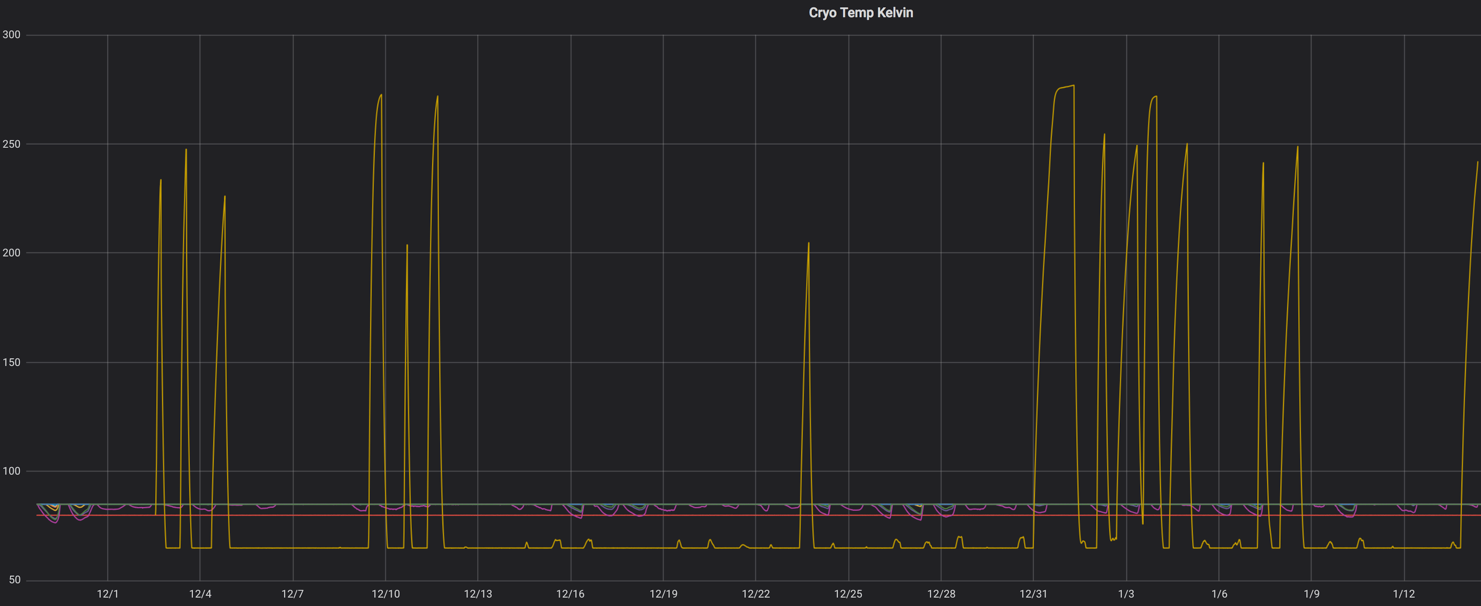
\includegraphics[width=1\linewidth]{../020" "(3C)/temperature-cycle.png}}
\caption{Grafana plot of the feed temperature during the test period.}
\label{fig:temperature-cycle}
\end{figure}
%
The inspection of the feed tip revealed that the prototype tip-link was still intact, and the failure was caused by the retraction of the center core of the coaxial cable.
The pictures of the inspection from the 14th of Jan 2020, are shown in Figure \ref{fig:inspect-020}. The log-periodic pyramid has been removed from the feed base and send to Minex, where the coaxial cable was removed and prepared for further X-RAY analysis.

\newpage
%
\begin{figure}[H]
   \thispagestyle{empty}
    \centering
        \begin{subfigure}[t]{0.92\textwidth}
        \centering
        \includegraphics[width=1\linewidth]{../020" "(3C)/3c-3.jpg}
        \caption{}
        \label{fig:Tsys-1g}
   	 \end{subfigure}
    %~
%        \begin{subfigure}[t]{0.475\textwidth}
%        \centering
%        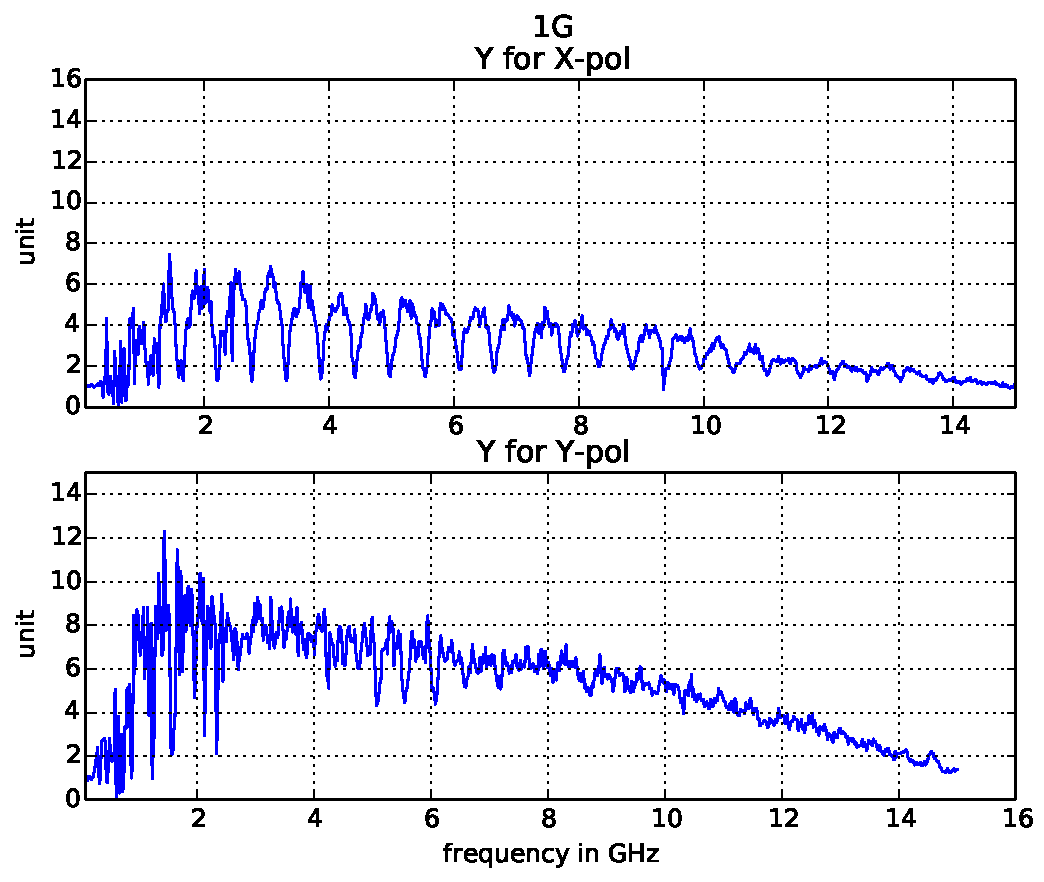
\includegraphics[width=1\linewidth]{figures/Antennas-10-2019/1g/Tsys/Y-factor.pdf}
%        \caption{Y-factor}
%        \label{fig:Y-factor-1g}
%   	\end{subfigure}
   
 	%\vspace{1mm}
   
        \begin{subfigure}[t]{0.92\textwidth}
        \centering
        \includegraphics[width=1\linewidth]{../020" "(3C)/3c-4.jpg}
        \caption{}
        \label{fig:SpecX-1g}
   	 \end{subfigure}
    %~
%        \begin{subfigure}[t]{0.475\textwidth}
%        \centering
%        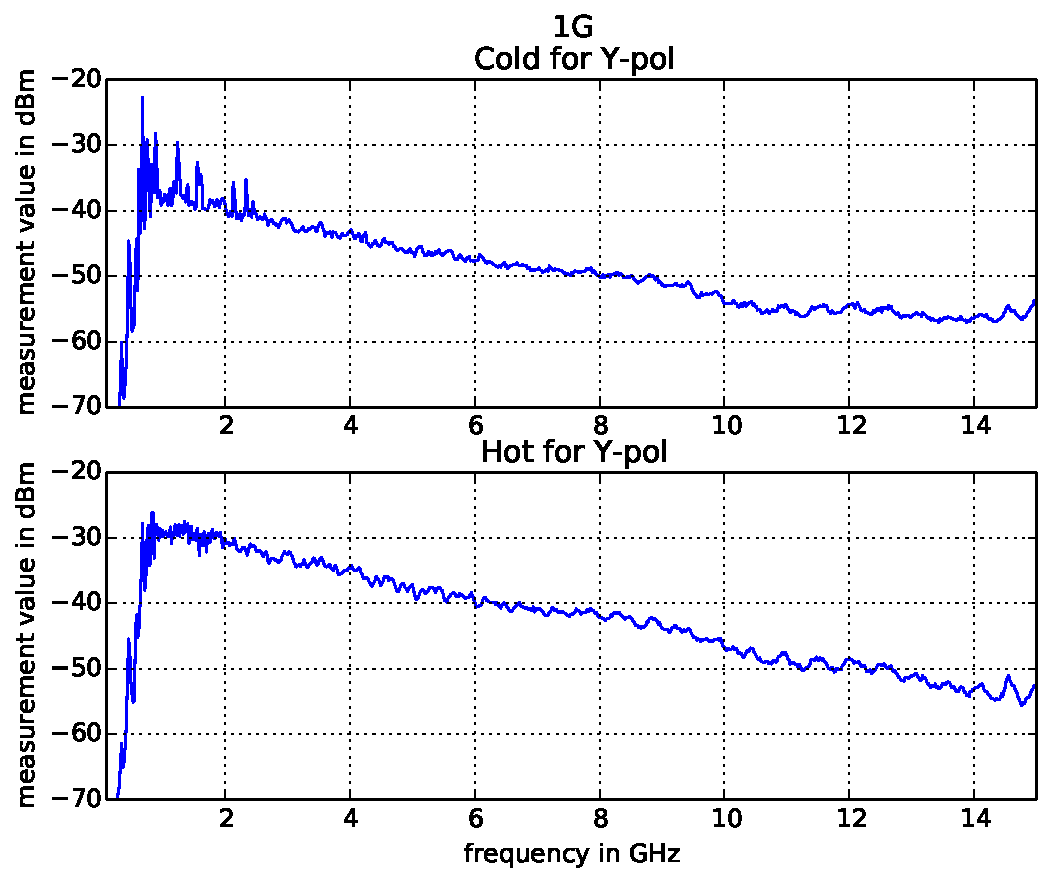
\includegraphics[width=1\linewidth]{figures/Antennas-10-2019/1g/Tsys/SpecY.pdf}
%        \caption{Spectrum Y-Polarization}
%        \label{fig:SpecY-1g}
%   	\end{subfigure}  
    %
    \caption{Tip of feed 020 previously installed on 3C. (a) Shows the left-hand side of the tip, which has a broken connection where the center conductor is permanently retracted. (b) Shows the right-hand side of the tip which is still intact. }
    \label{fig:inspect-020}
\end{figure}
%









\newpage
\section{Feed 006 (4J)\\ $[$wiring harness replaced at HCRO$]$}
\label{sec:3}
% ----------------------------------------------------------------

This feed was selected for a retrofit with a revised wiring harness at HCRO in 2019. After the modified wiring harness was installed we discovered inconsistencies
in the LNA bias supply wiring, which is specific to this feed. Therefore, the log-periodic pyramid and feed base are unique and can not be interchanged with other feed bases or log-periodic pyramids. As part of the repair which will happen on this feed we will investigate to fix the wiring of the LNAs and change it to the standard configuration that is used in all other Antonio Feeds.

The inspection of the feed tip revealed that the original tip-link was still intact, and the failure was caused by the retraction of the center core of the coaxial cable.
The pictures of the inspection from the 17th of Feb 2020, are shown in Figure \ref{fig:inspect-020(0)}  and \ref{fig:inspect-020(1)}. The log-periodic pyramid has been removed from the feed base and will be disassembled in order to inspect the LNA end of the coaxial cable.

%
\begin{figure}[H]
\centering{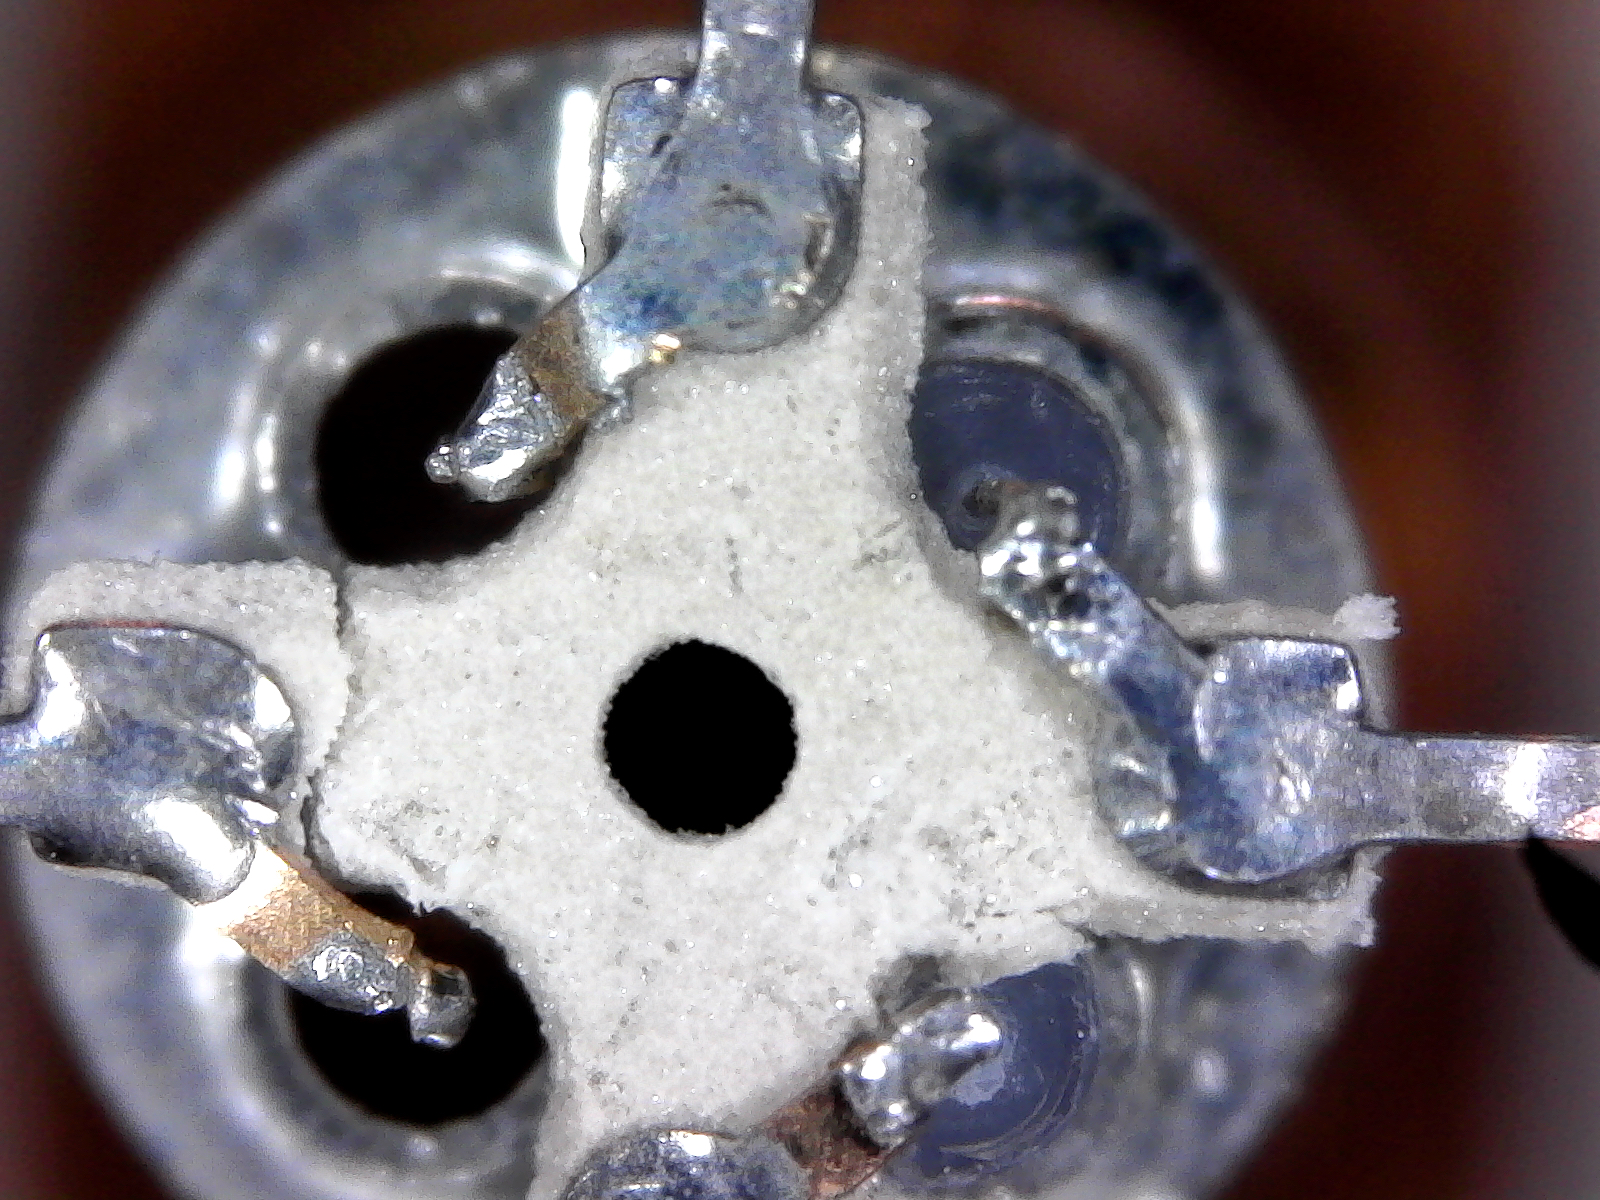
\includegraphics[width=0.89\linewidth]{../006" "(4J)/4J-2.jpg}}
\caption{Top view of the tip of feed 006, previously installed on 4J. One can see that on the left-hand side both coaxial cable center conductor are retracted. The lower left coaxial cable broke off and even caused the capacitor board to break.}
\label{fig:inspect-020(0)}
\end{figure}
%


\newpage
%
\begin{figure}[H]
   \thispagestyle{empty}
    \centering
        \begin{subfigure}[t]{0.92\textwidth}
        \centering
        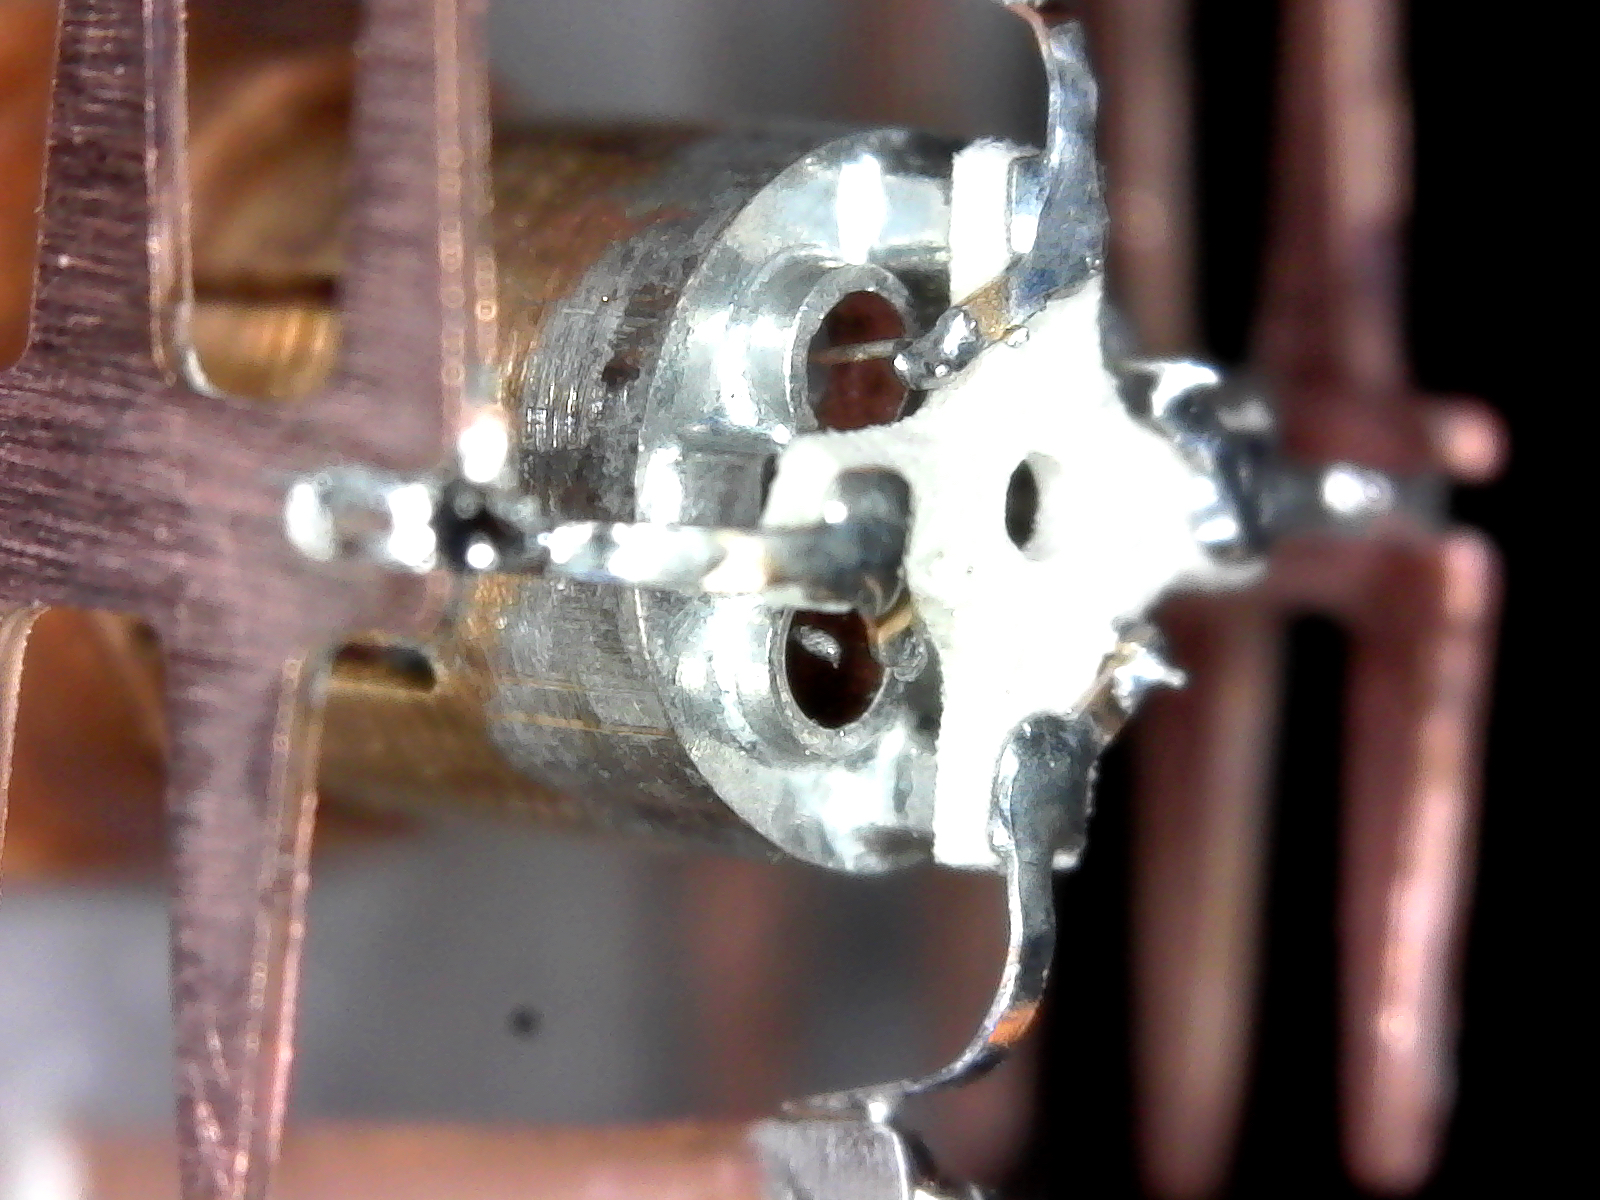
\includegraphics[width=1\linewidth]{../006" "(4J)/4J-0.jpg}
        \caption{}
        \label{fig:Tsys-1g}
   	 \end{subfigure}
    %~
%        \begin{subfigure}[t]{0.475\textwidth}
%        \centering
%        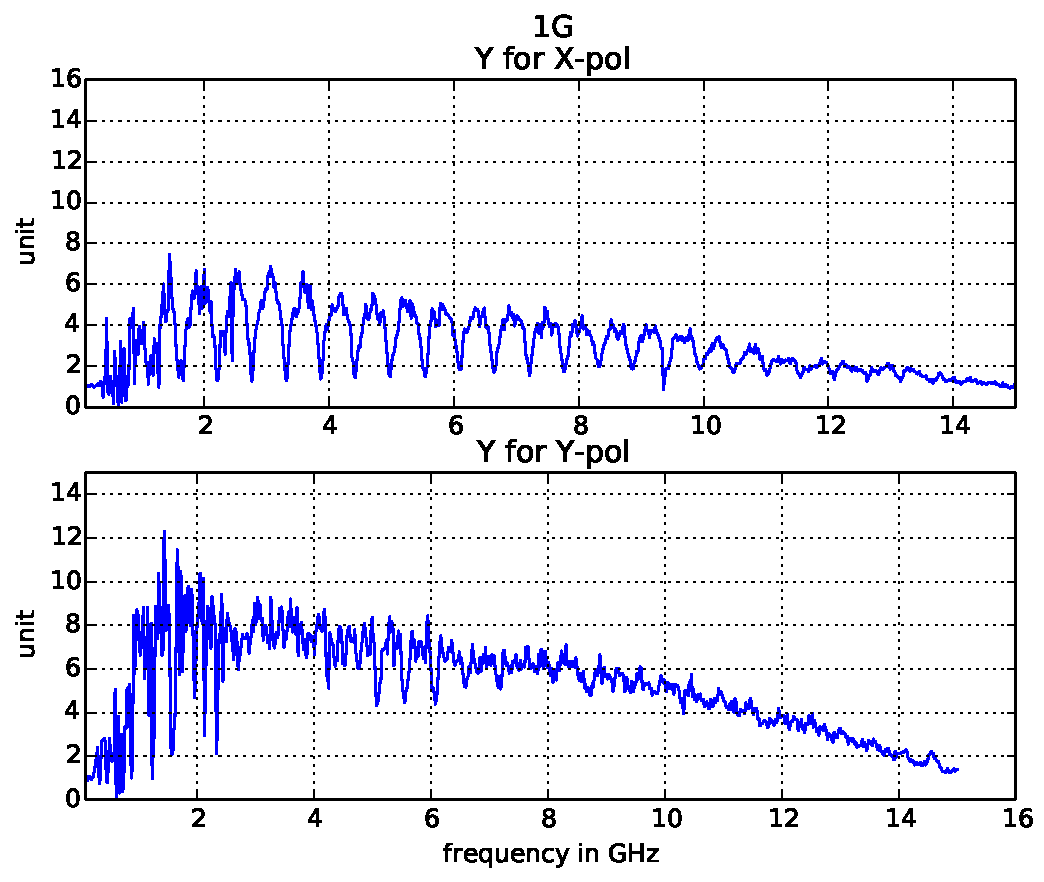
\includegraphics[width=1\linewidth]{figures/Antennas-10-2019/1g/Tsys/Y-factor.pdf}
%        \caption{Y-factor}
%        \label{fig:Y-factor-1g}
%   	\end{subfigure}
   
 	%\vspace{1mm}
   
        \begin{subfigure}[t]{0.92\textwidth}
        \centering
        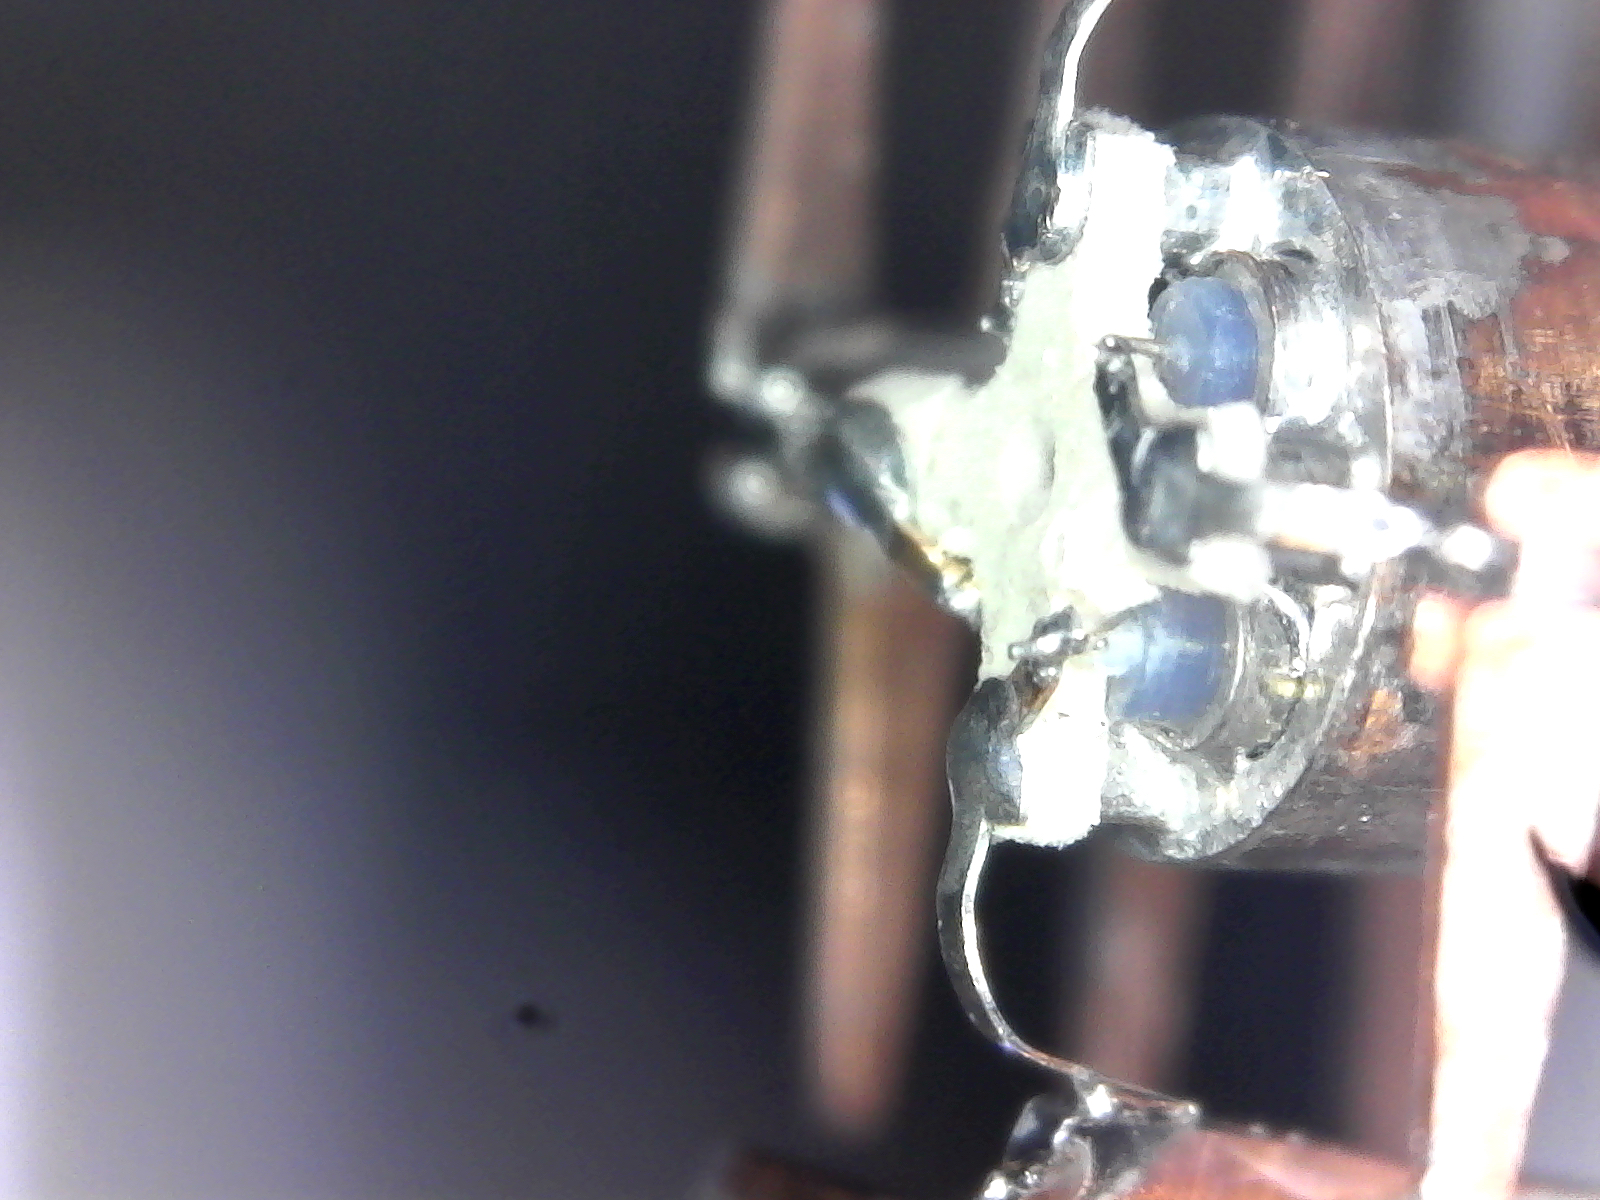
\includegraphics[width=1\linewidth]{../006" "(4J)/4J-1.jpg}
        \caption{}
        \label{fig:SpecX-1g}
   	 \end{subfigure}
    %~
%        \begin{subfigure}[t]{0.475\textwidth}
%        \centering
%        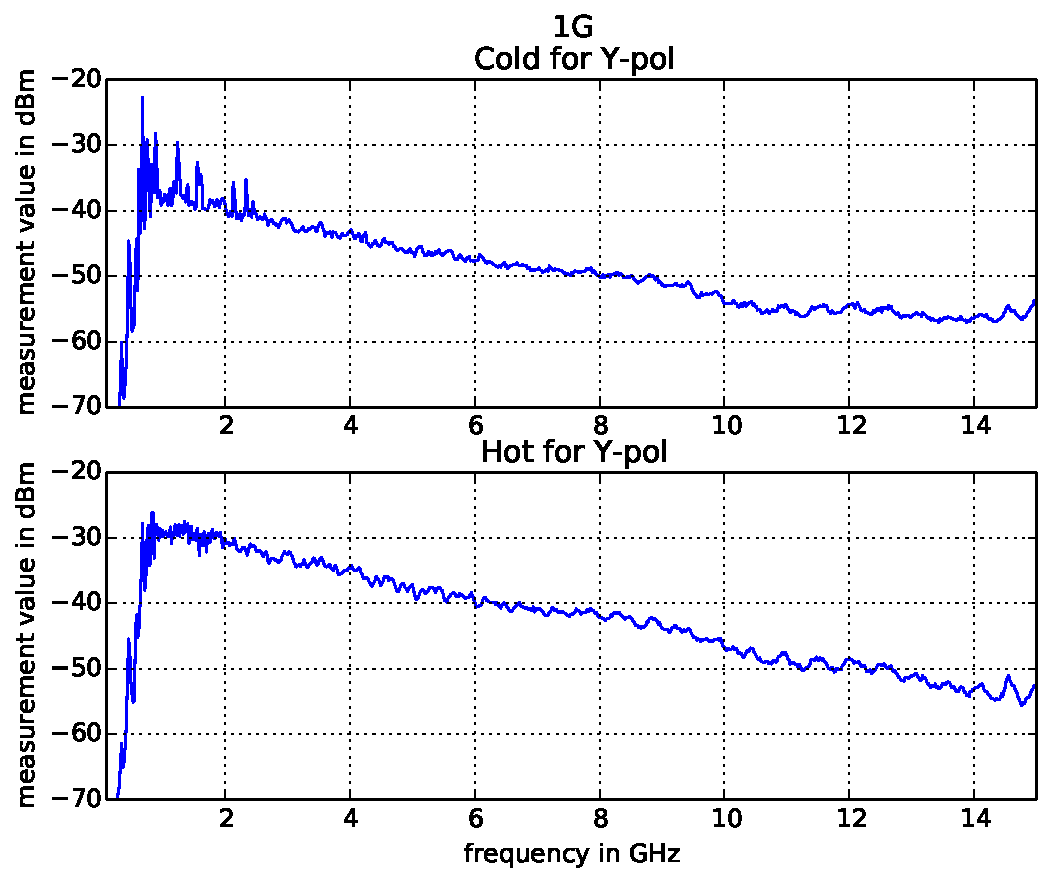
\includegraphics[width=1\linewidth]{figures/Antennas-10-2019/1g/Tsys/SpecY.pdf}
%        \caption{Spectrum Y-Polarization}
%        \label{fig:SpecY-1g}
%   	\end{subfigure}  
    %
    \caption{Tip of feed 006 previously installed on 4J. (a) Shows the left-hand side of the tip, which has a broken connection where the center conductor is permanently retracted. (b) Shows the right-hand side of the tip which is still intact. }
    \label{fig:inspect-020(1)}
\end{figure}



\section{Feed 013 (1H)\\$[$original Antonio Feed$]$}
\label{sec:4}
% ----------------------------------------------------------------

This feed is an original Antonio Feed with no modifications or retrofitted components. The feed has been identified as non operational during the feed system temperature measurements in Oct. 2019 and was switched off afterwards. As part of the tip failure investigation this feed was removed from antenna 1H and inspected. The overall condition of the log-periodic pyramid is shown in Figure \ref{fig:inspect-013(0)}. One can see that there is some amount of dust and particles located at the bottom of the base plate, as well as dust on the log-periodic pyramid itself. The inspection showed that the Rexolite fixture of the feed arms degraded by the vibrations of the cryocooler.

The inspection of the feed tip is shown in Figure \ref{fig:inspect-013(1)}. One can see that the failure of this feed is caused by a combination of coaxial center conductor retraction and broken tip-link connections to the feed arm. As this is a non retrofitted feed, it is very likely that the cryocooler is not tuned and therefore the vibrations experienced by the log-periodic feed were higher than in the revised feed versions.


\newpage
%
\begin{figure}[H]
   %\thispagestyle{empty}
    \centering
        \begin{subfigure}[t]{0.475\textwidth}
        \centering
        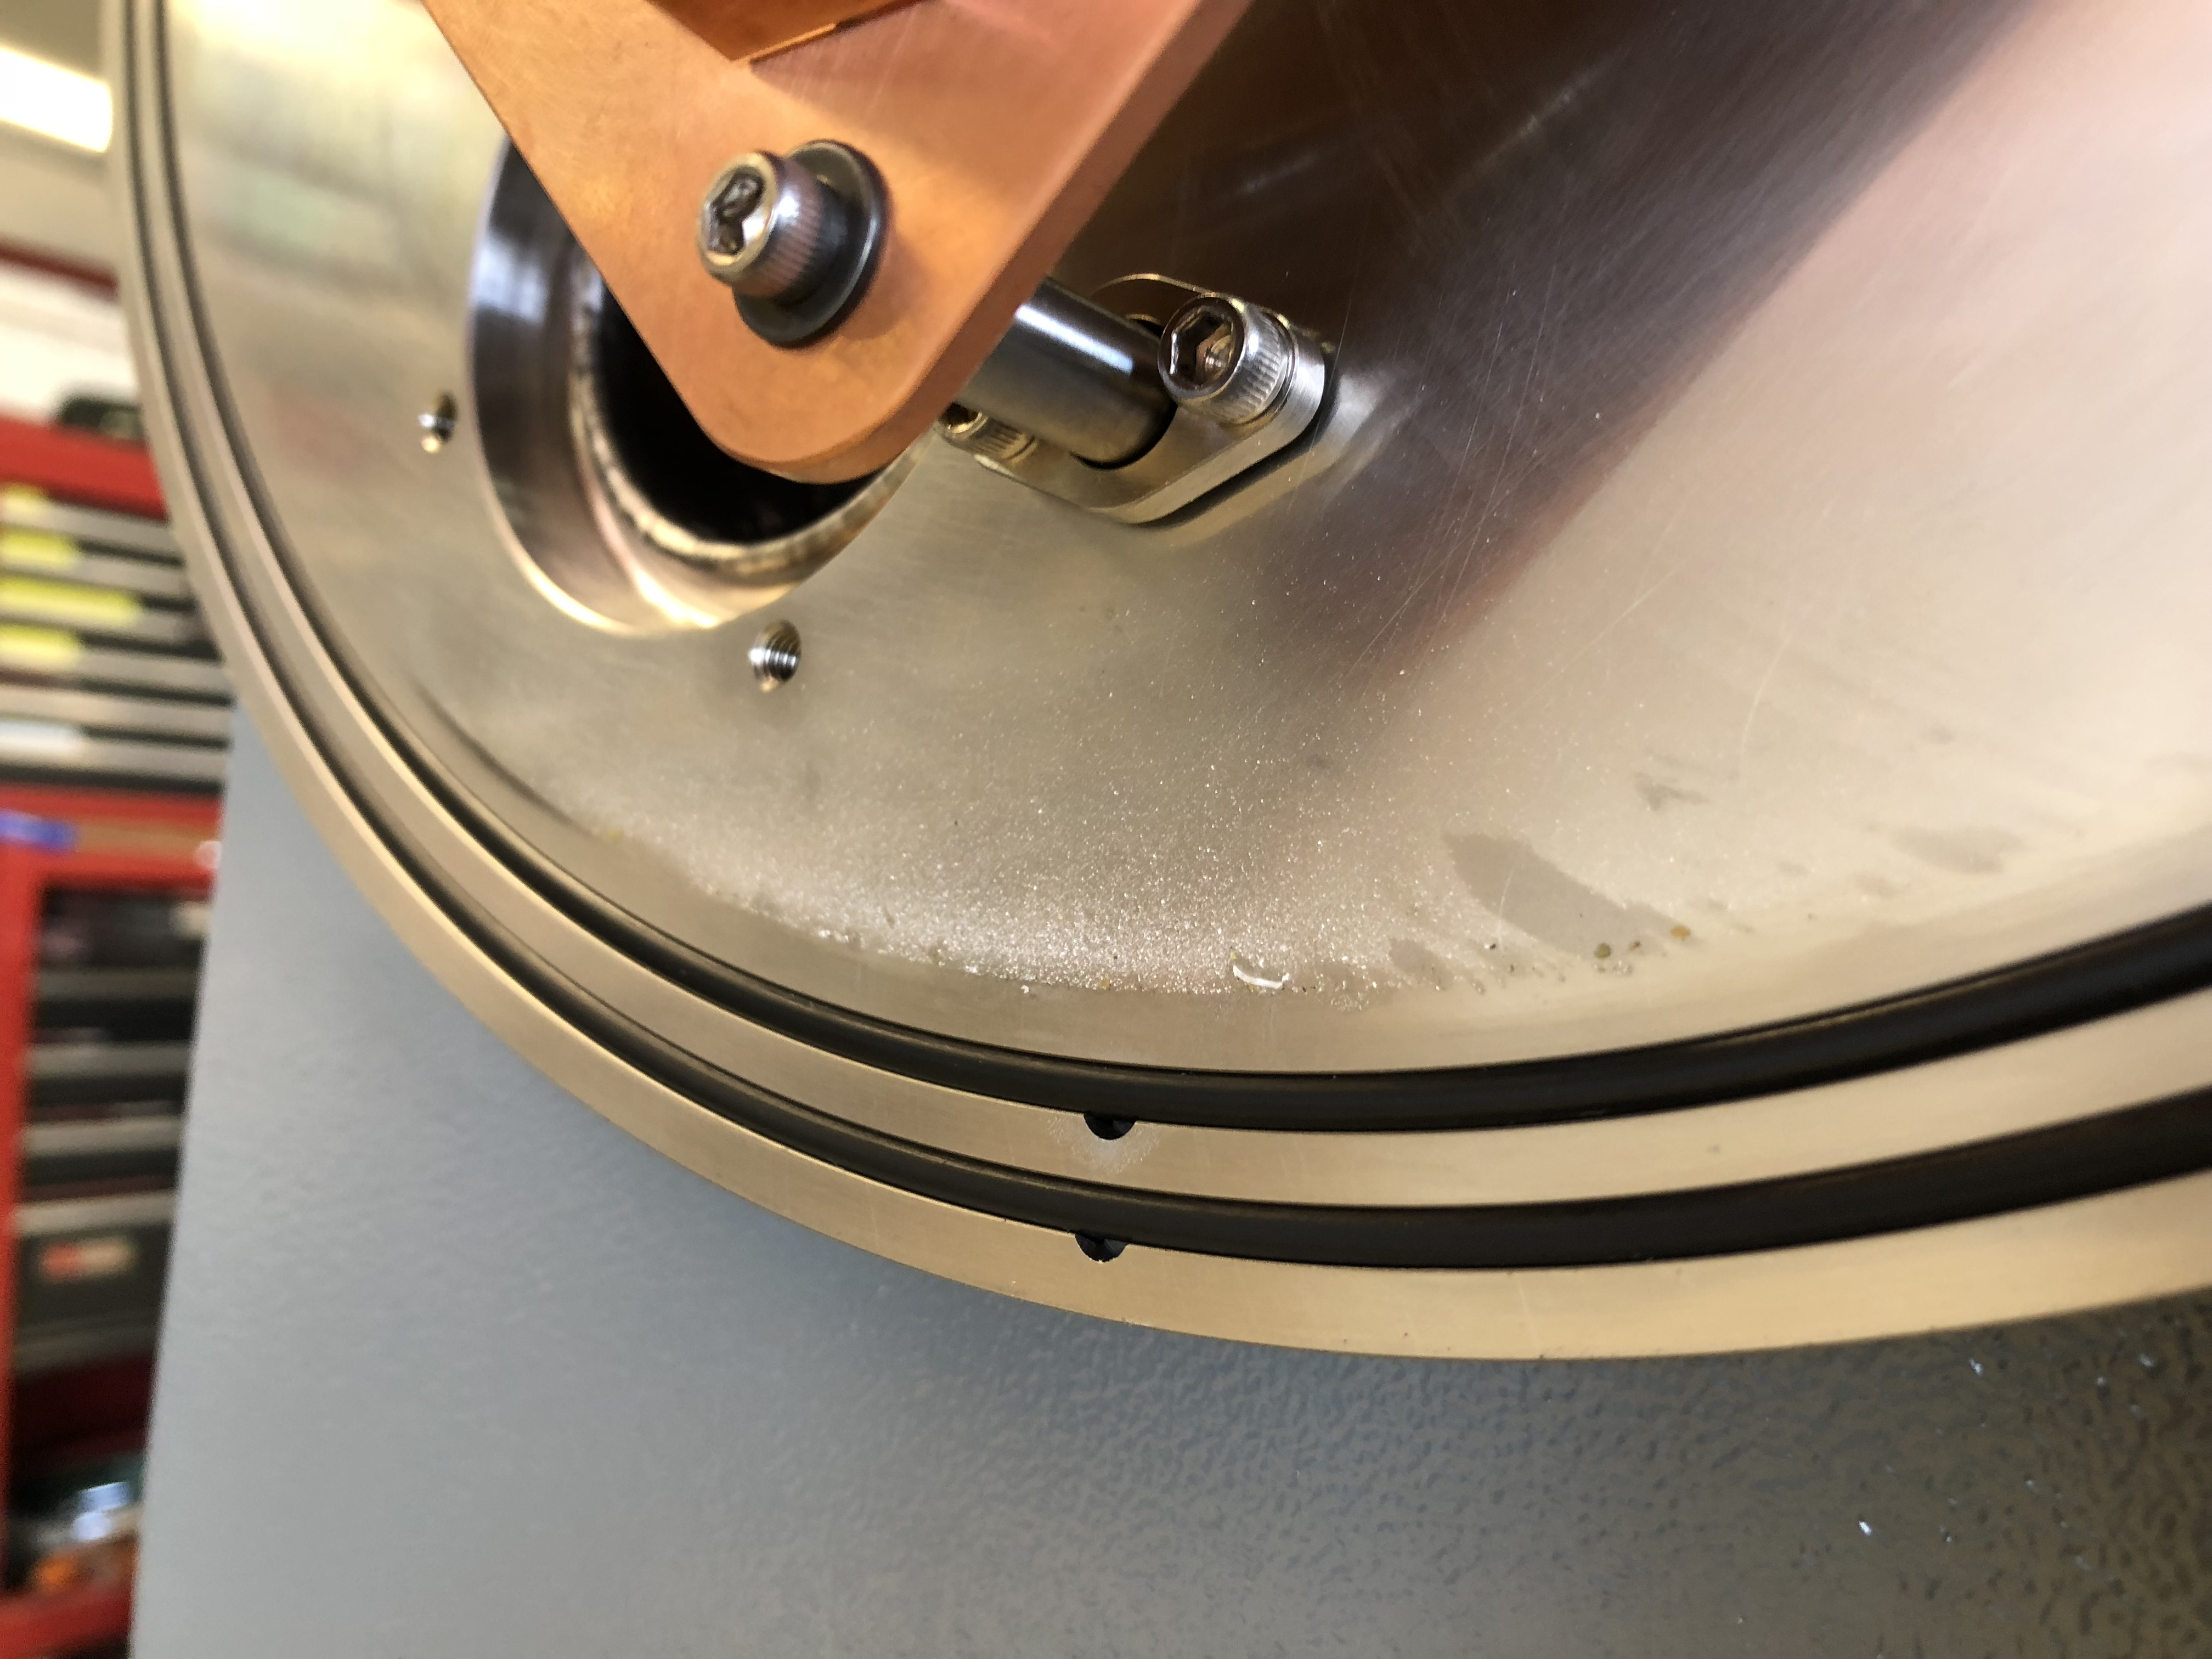
\includegraphics[width=1\linewidth]{../013" "(1H)/IMG_5289.jpg}
        \caption{}
        \label{fig:}
   	 \end{subfigure}
    %~
        \begin{subfigure}[t]{0.475\textwidth}
        \centering
        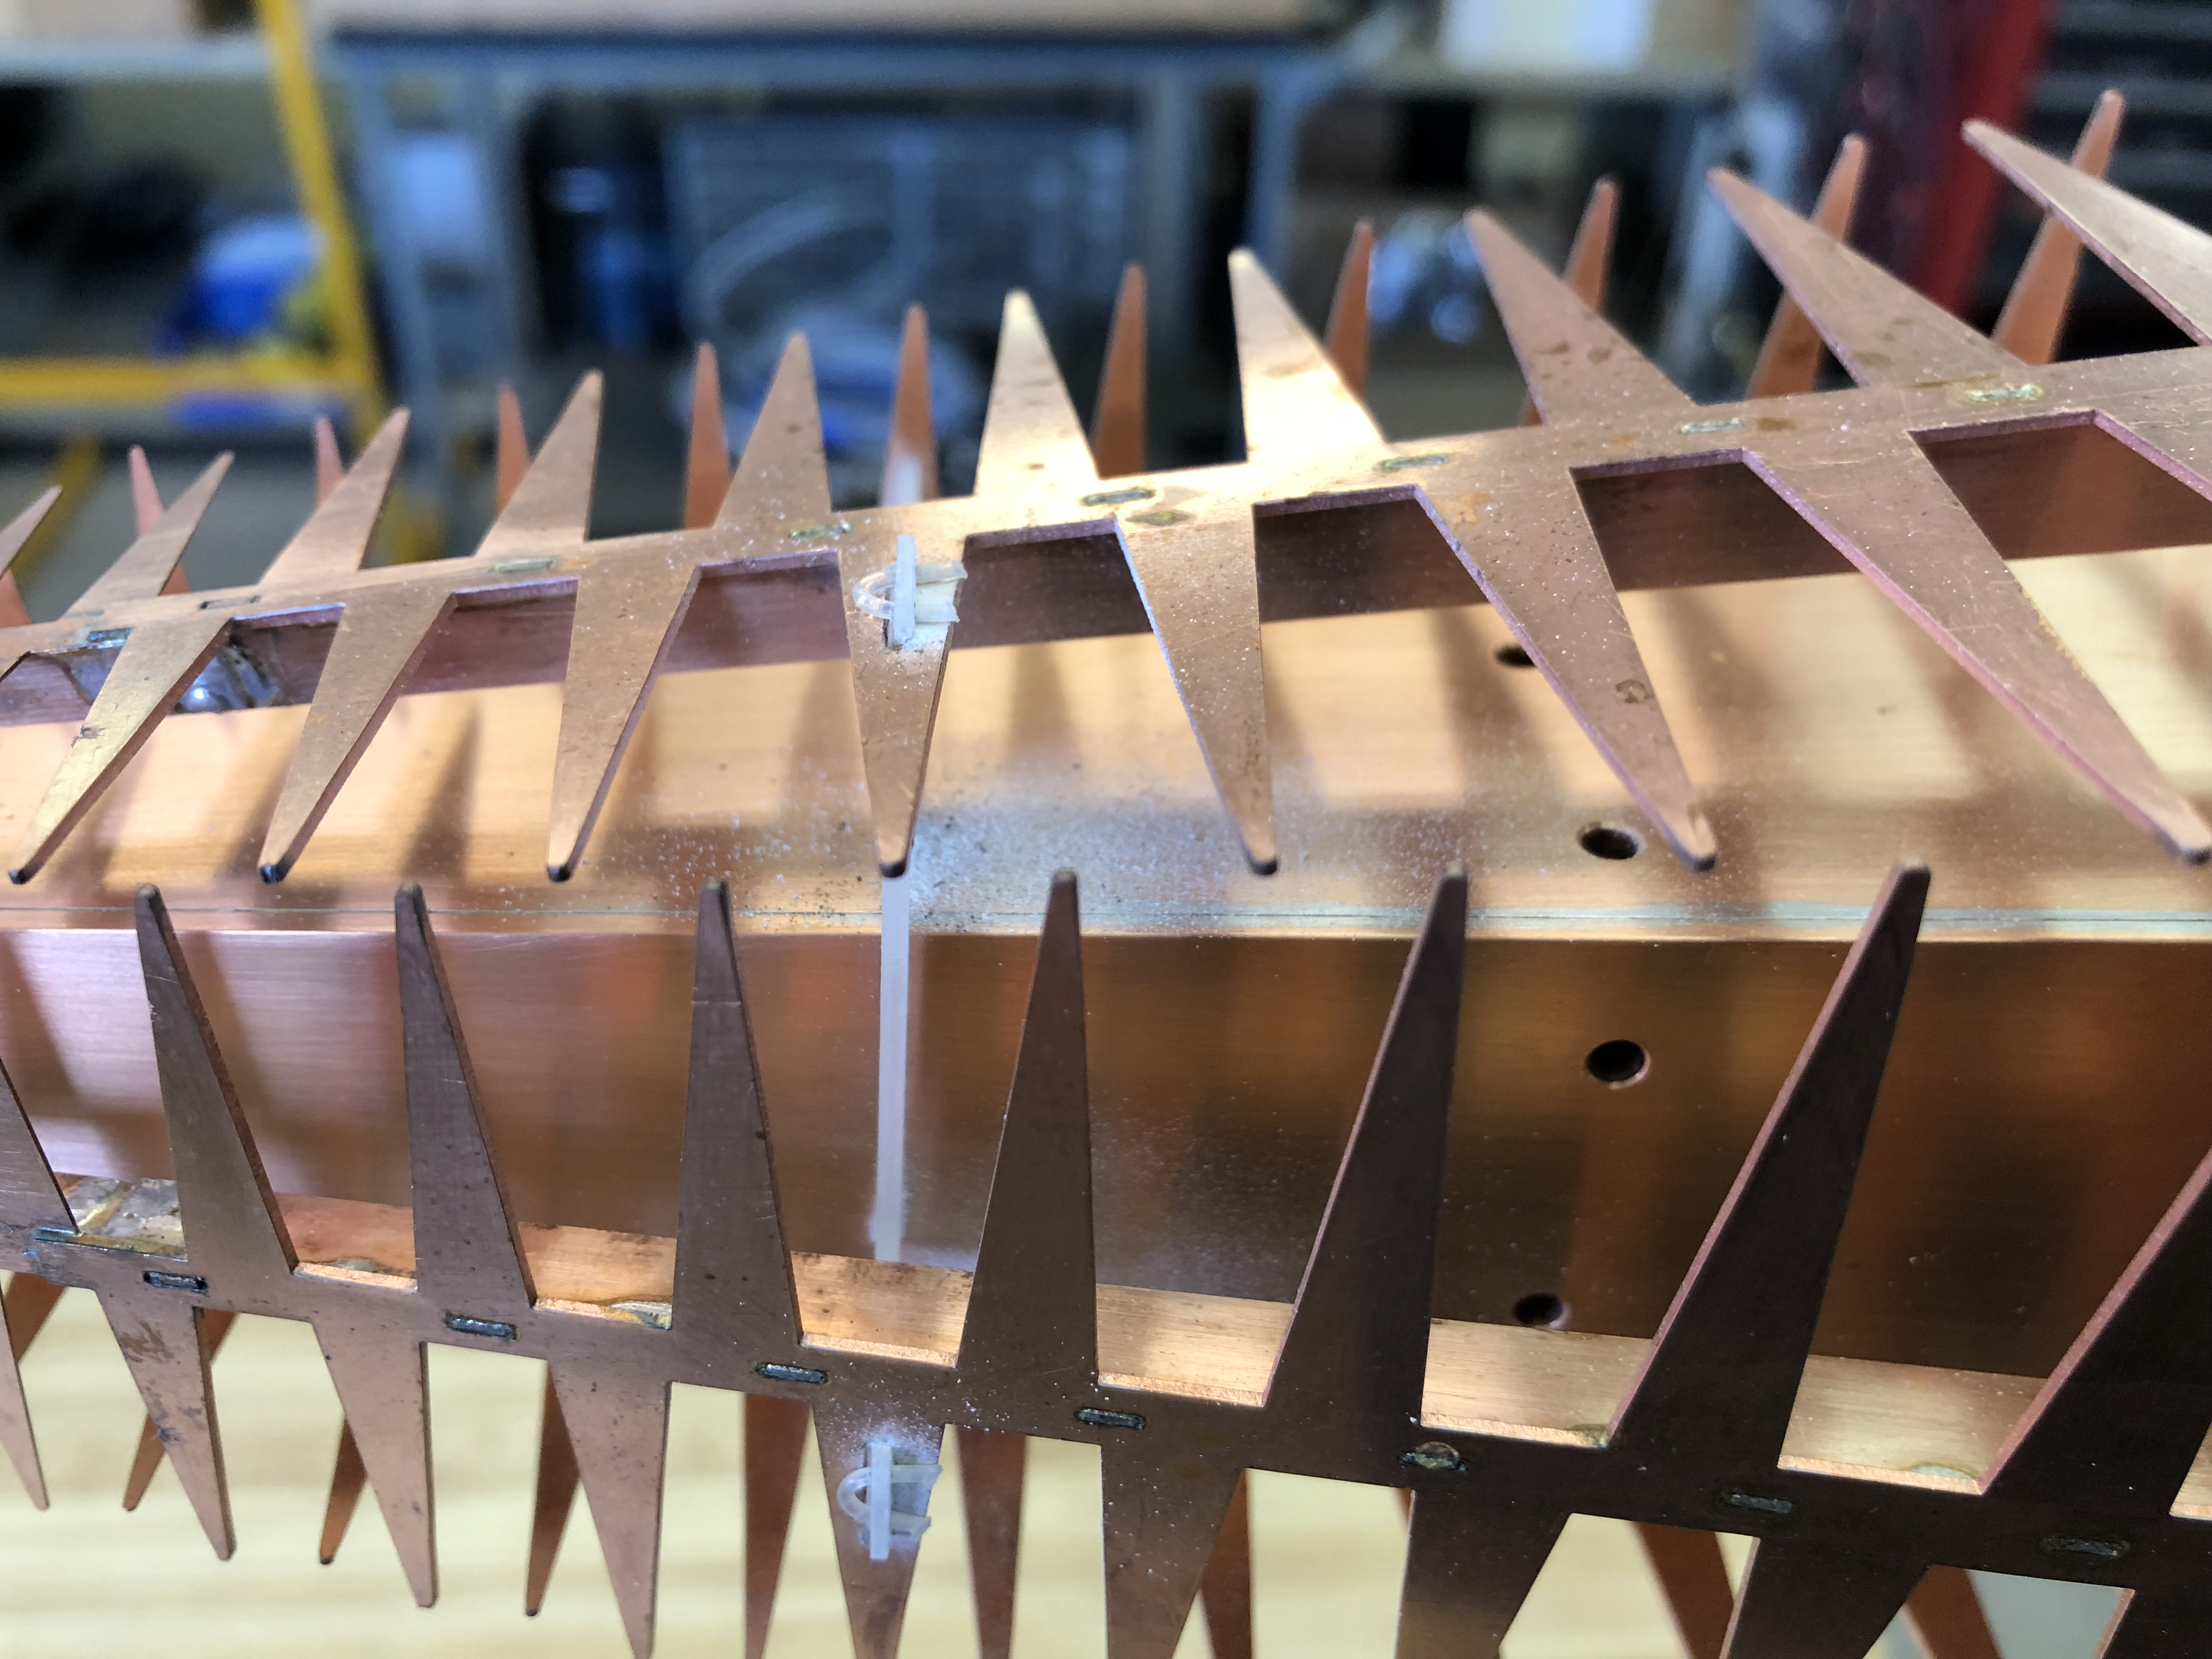
\includegraphics[width=1\linewidth]{../013" "(1H)/IMG_5292.jpg}
        \caption{}
        \label{fig:}
   	\end{subfigure}
   
 	\vspace{1mm}
   
        \begin{subfigure}[t]{0.475\textwidth}
        \centering
        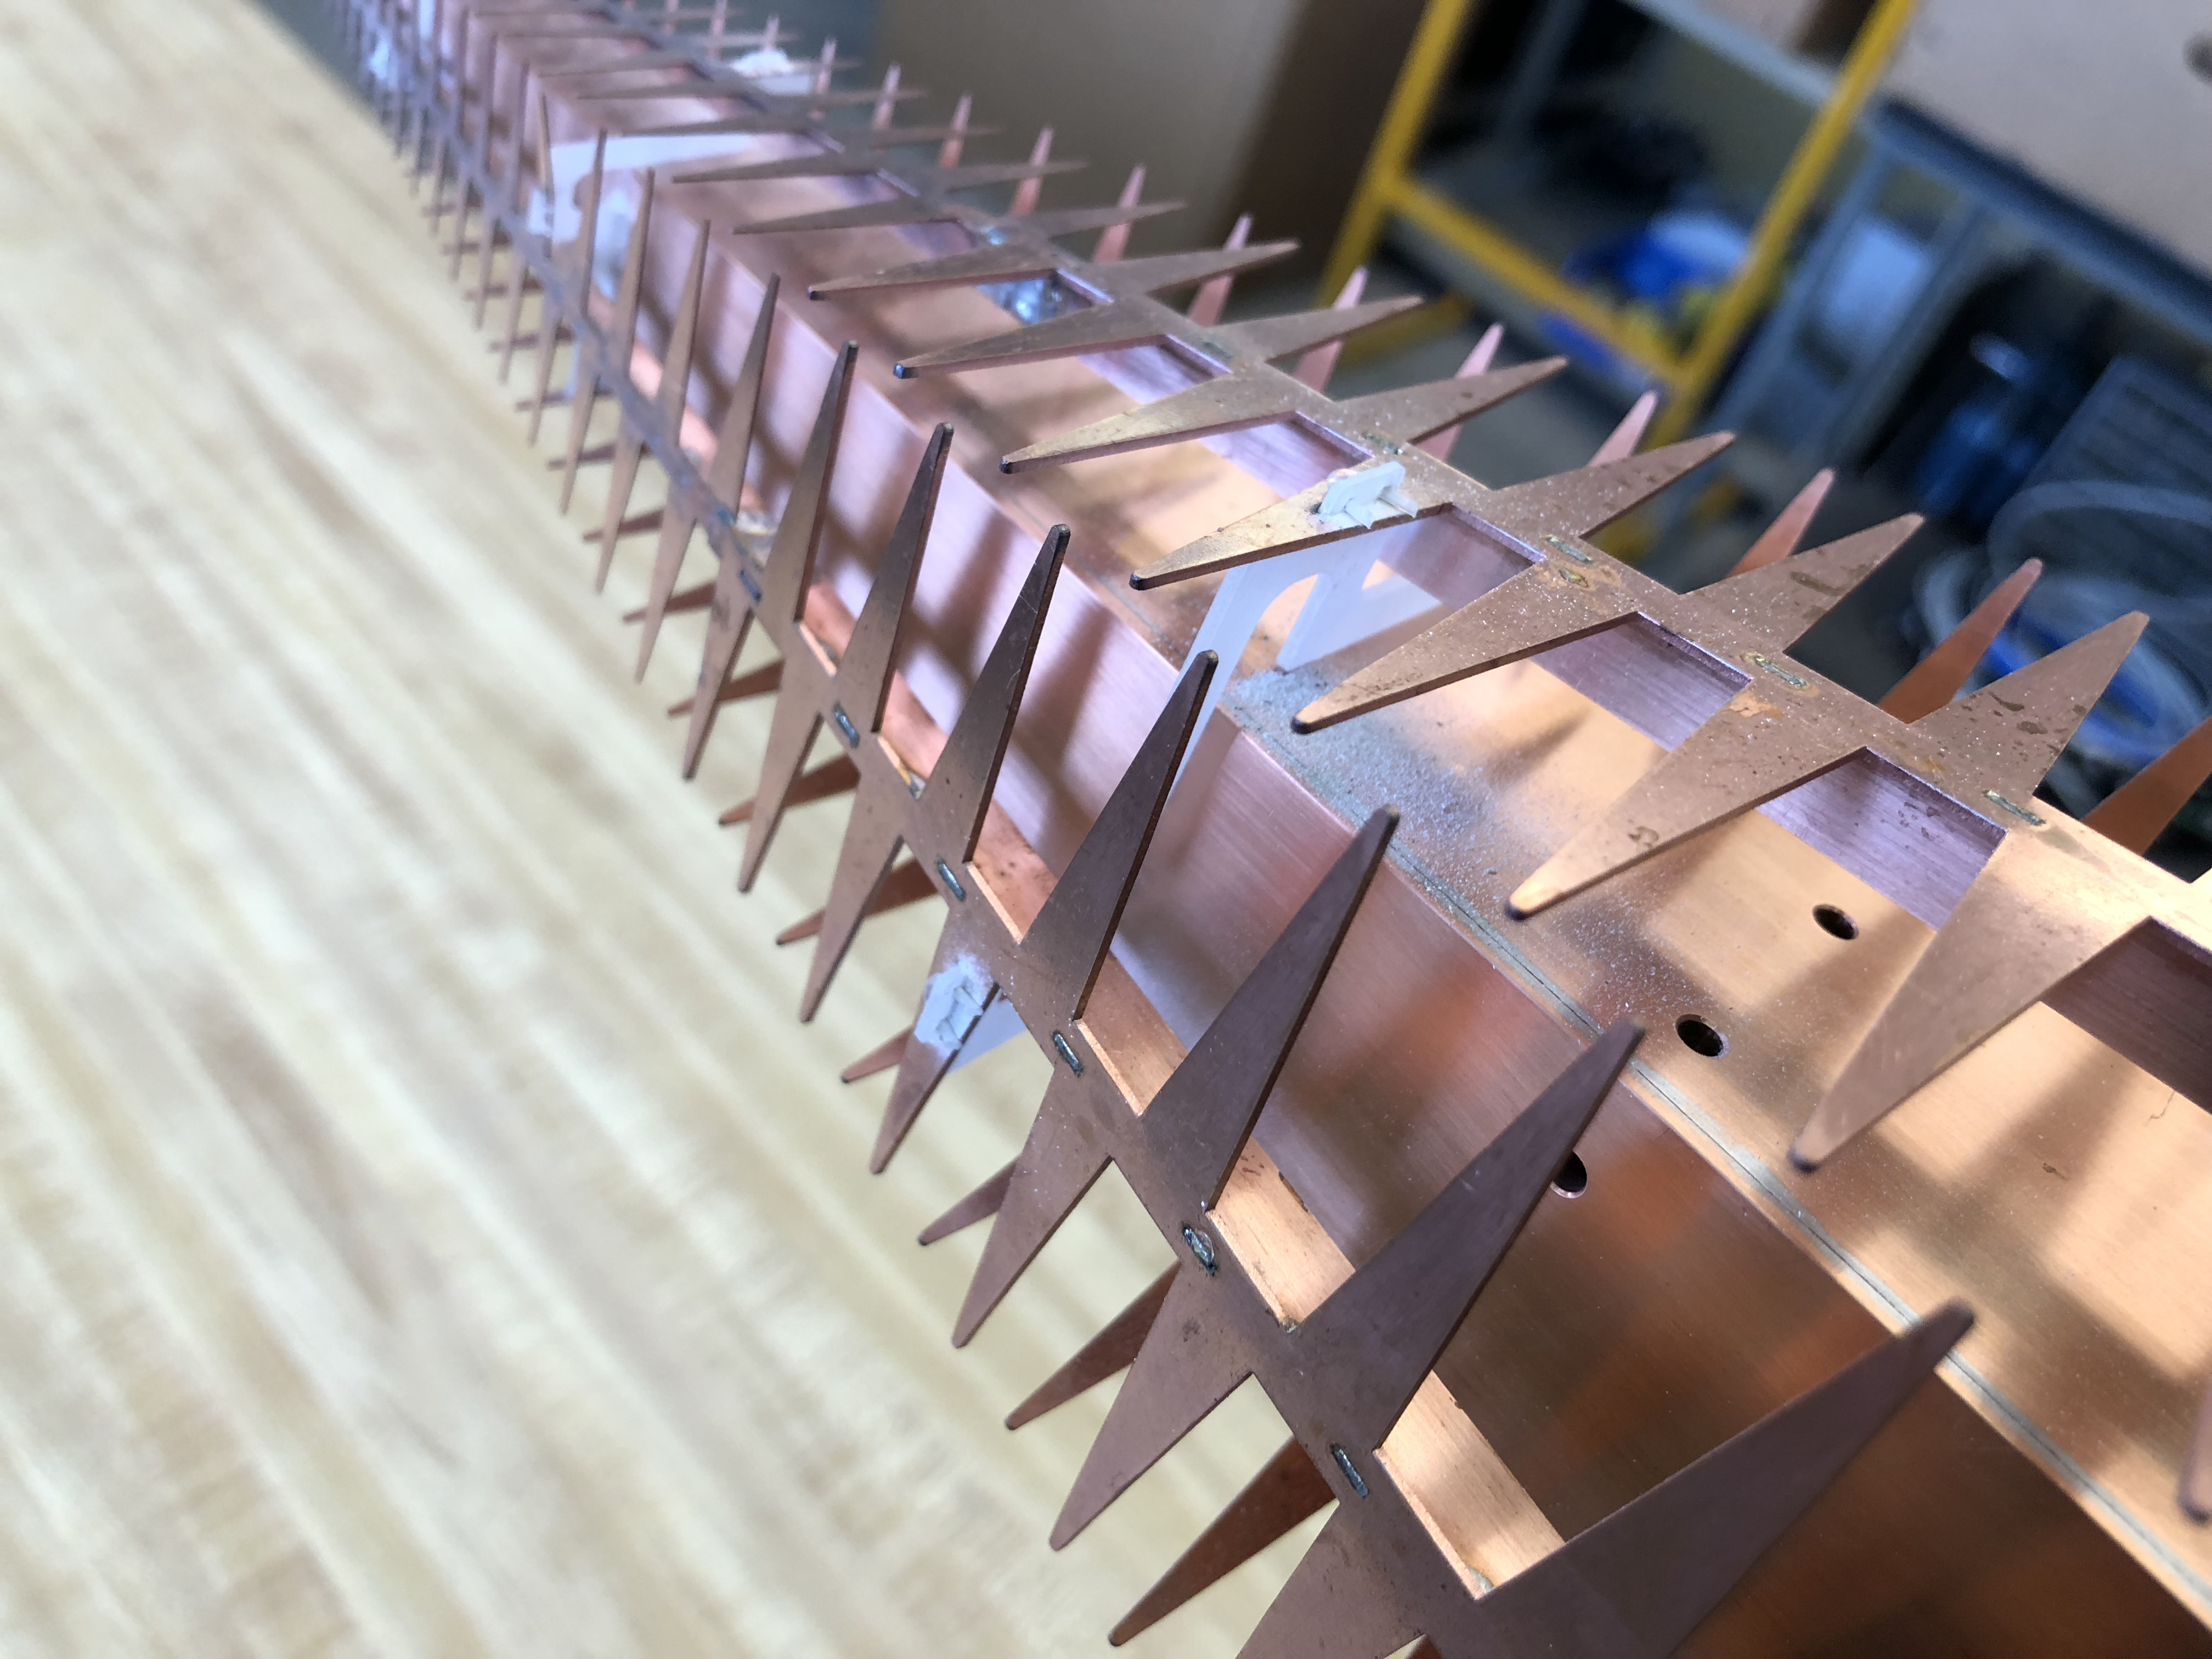
\includegraphics[width=1\linewidth]{../013" "(1H)/IMG_5293.jpg}
        \caption{}
        \label{fig:}
   	 \end{subfigure}
    %~
        \begin{subfigure}[t]{0.475\textwidth}
        \centering
        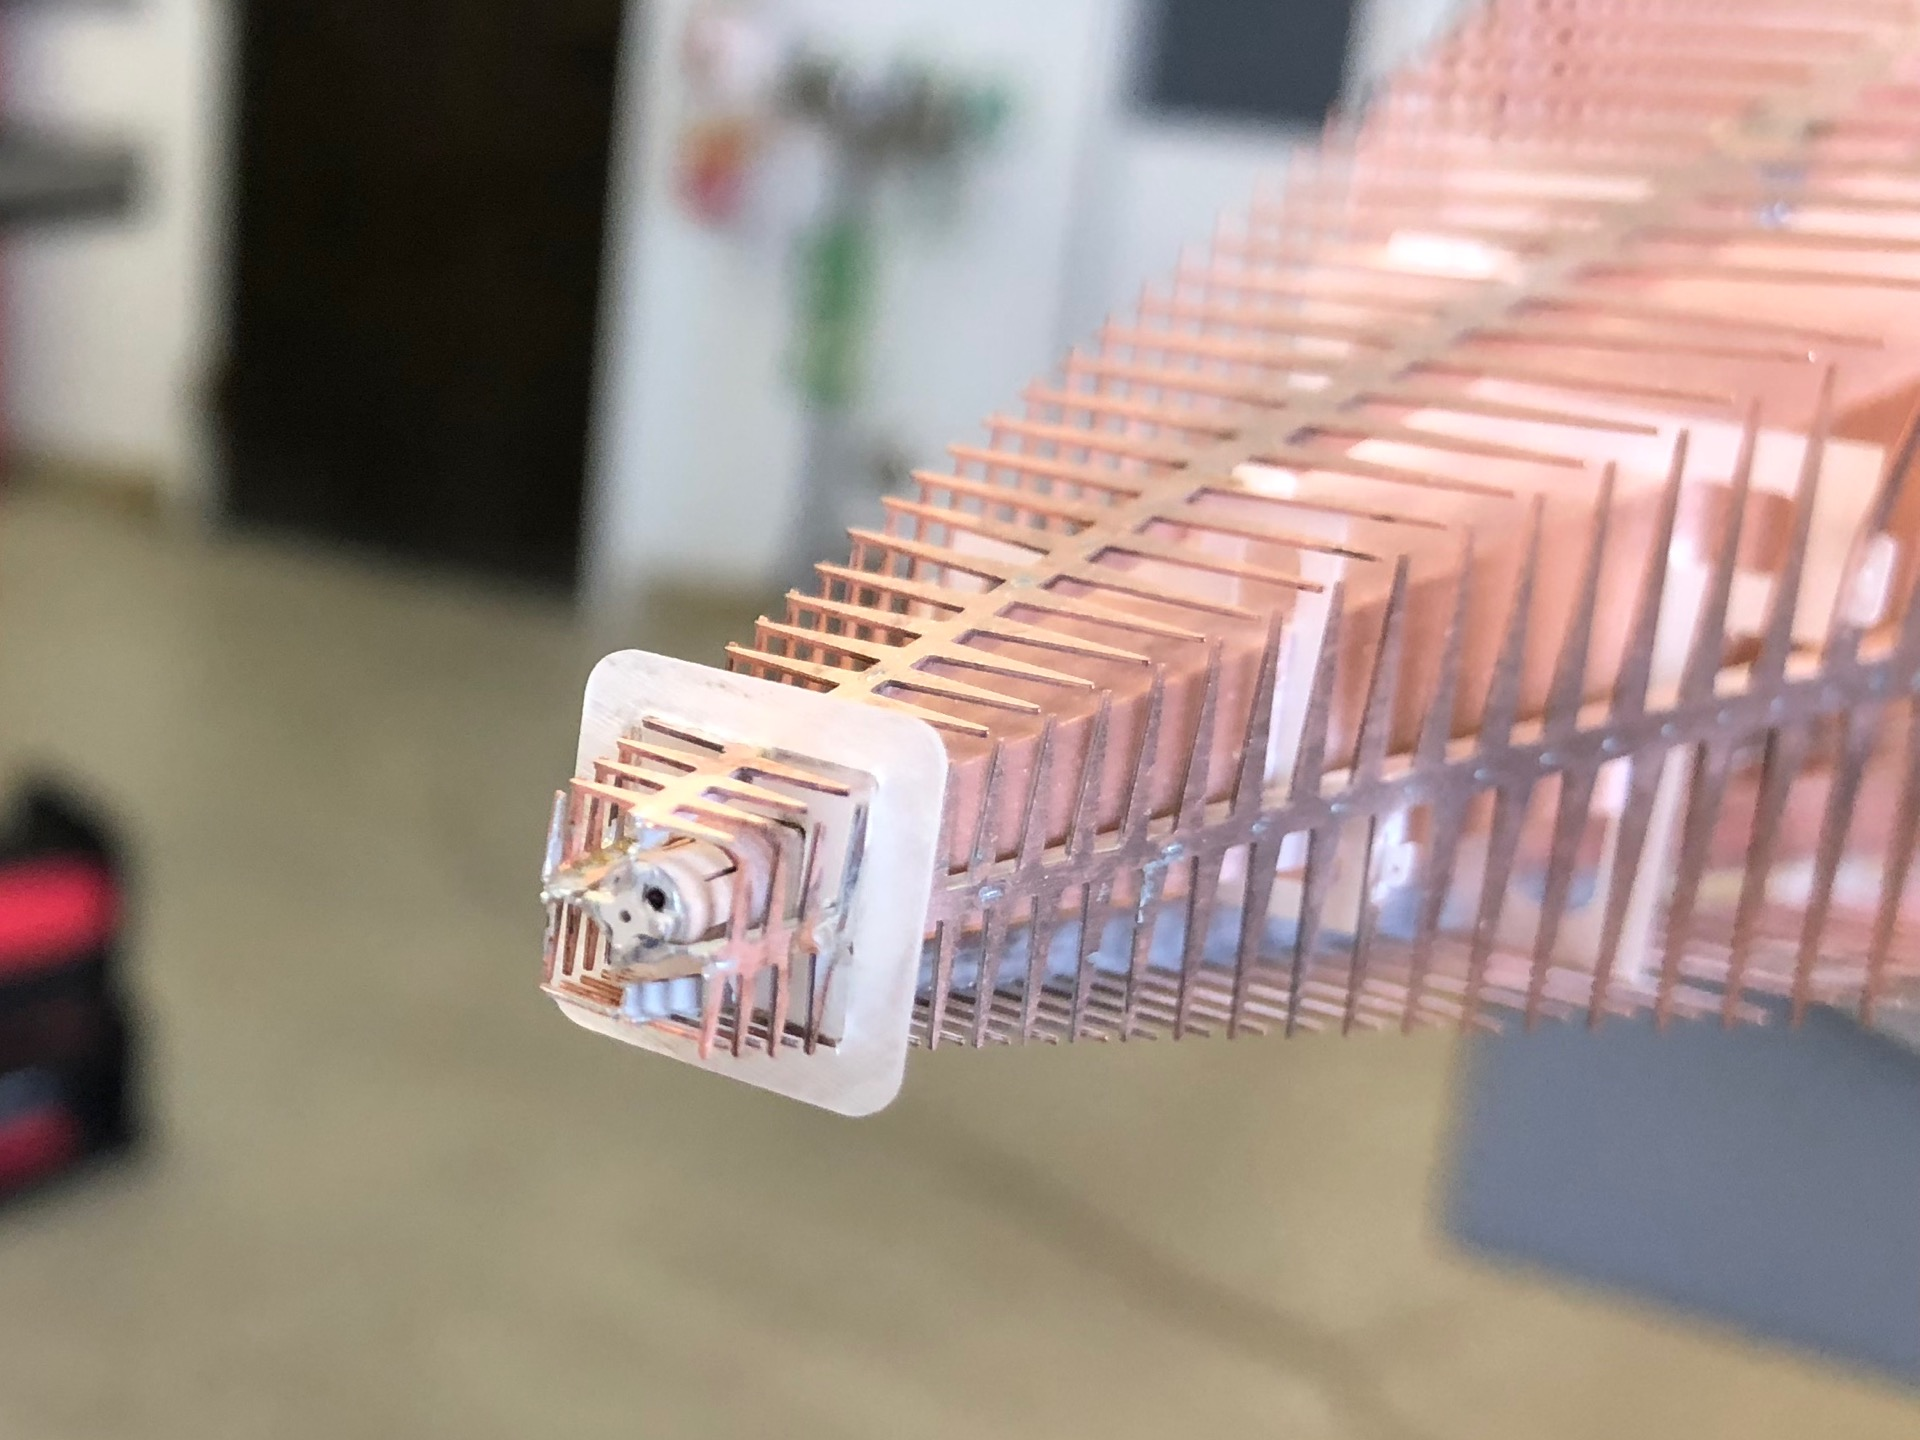
\includegraphics[width=1\linewidth]{../013" "(1H)/IMG_5295-2.jpg}
        \caption{}
        \label{fig:}
  	\end{subfigure}  
    %
    \caption{Inspection of the cryostat and log-periodic pyramid of feed 013 (1H). (a) Shows the bottom of the base plate of the cryostat, which is contaminated by white dust and other particles. (b) and (c) Show the wear of the Rexolite standoffs caused by the vibration of the log-periodic pyramid structure (white dust). (d) Shows the tip, which also has white dust on it. }
    \label{fig:inspect-013(0)}
\end{figure}


\newpage
%
\begin{figure}[H]
   %\thispagestyle{empty}
    \centering
        \begin{subfigure}[t]{0.475\textwidth}
        \centering
        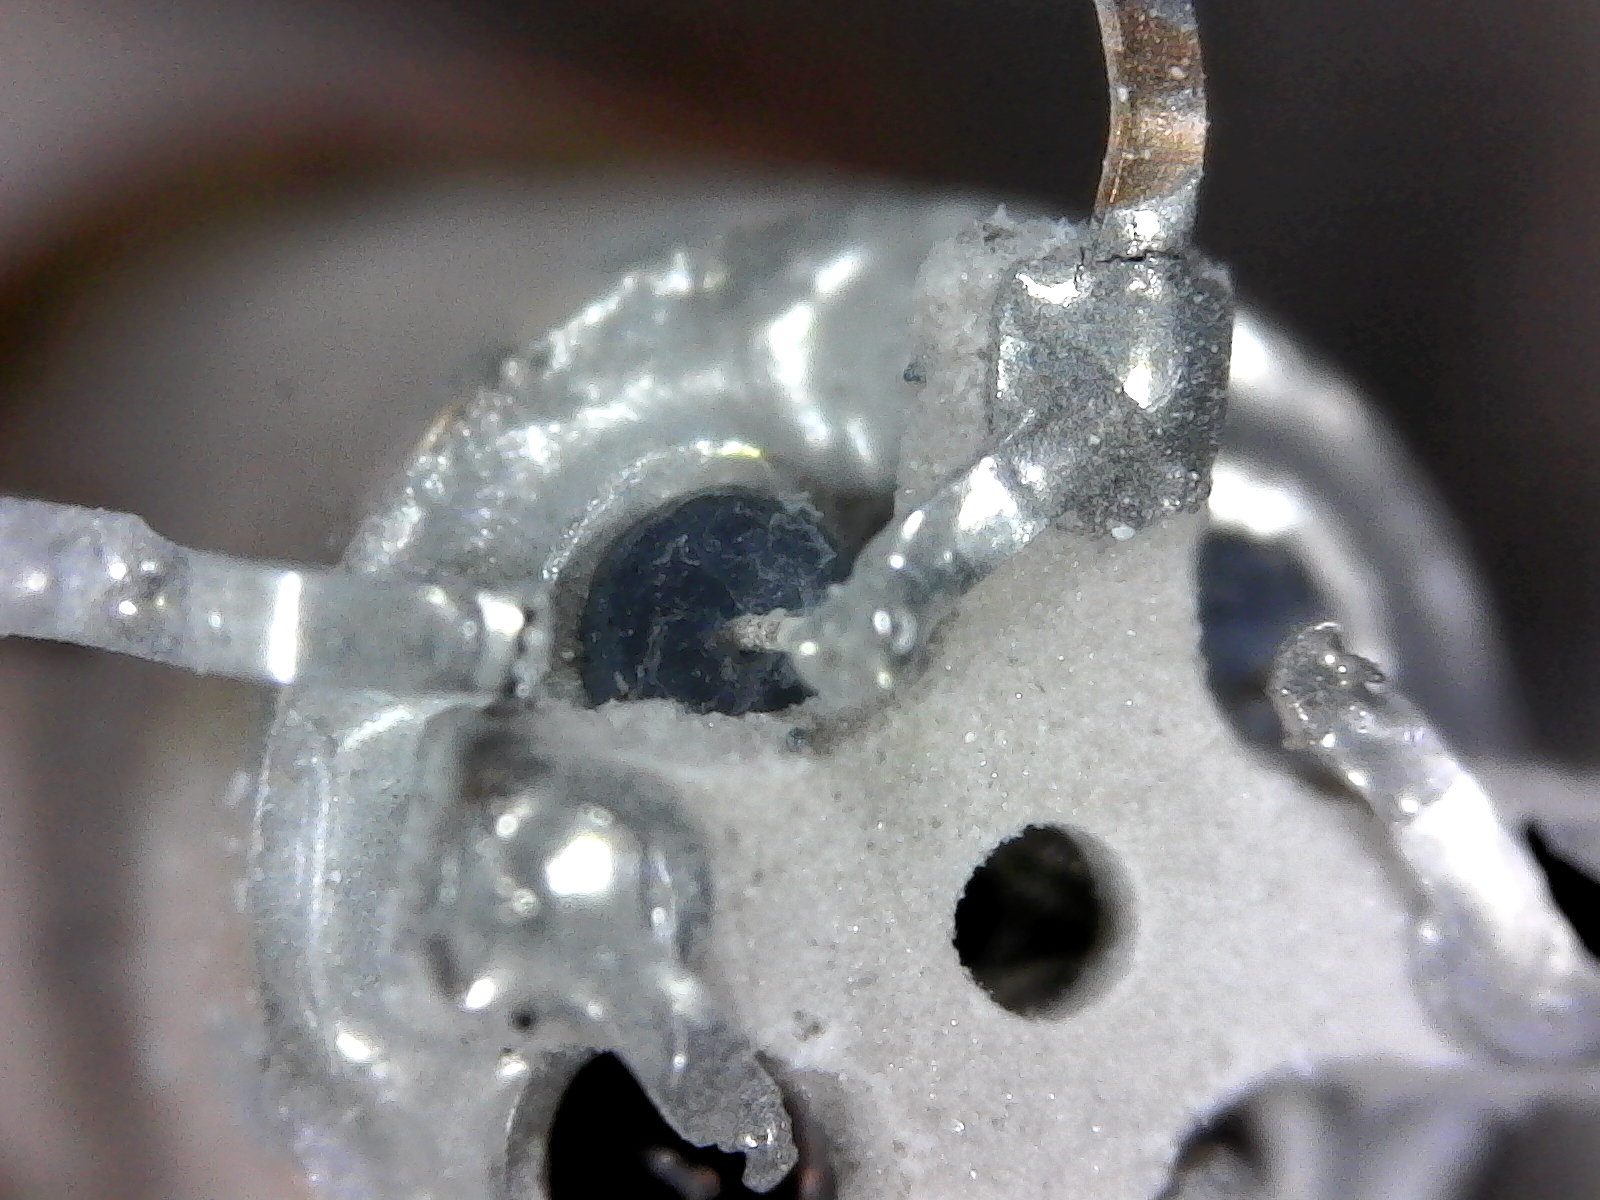
\includegraphics[width=1\linewidth]{../013" "(1H)/1H-1.jpg}
        \caption{}
        \label{fig:}
   	 \end{subfigure}
    %~
        \begin{subfigure}[t]{0.475\textwidth}
        \centering
        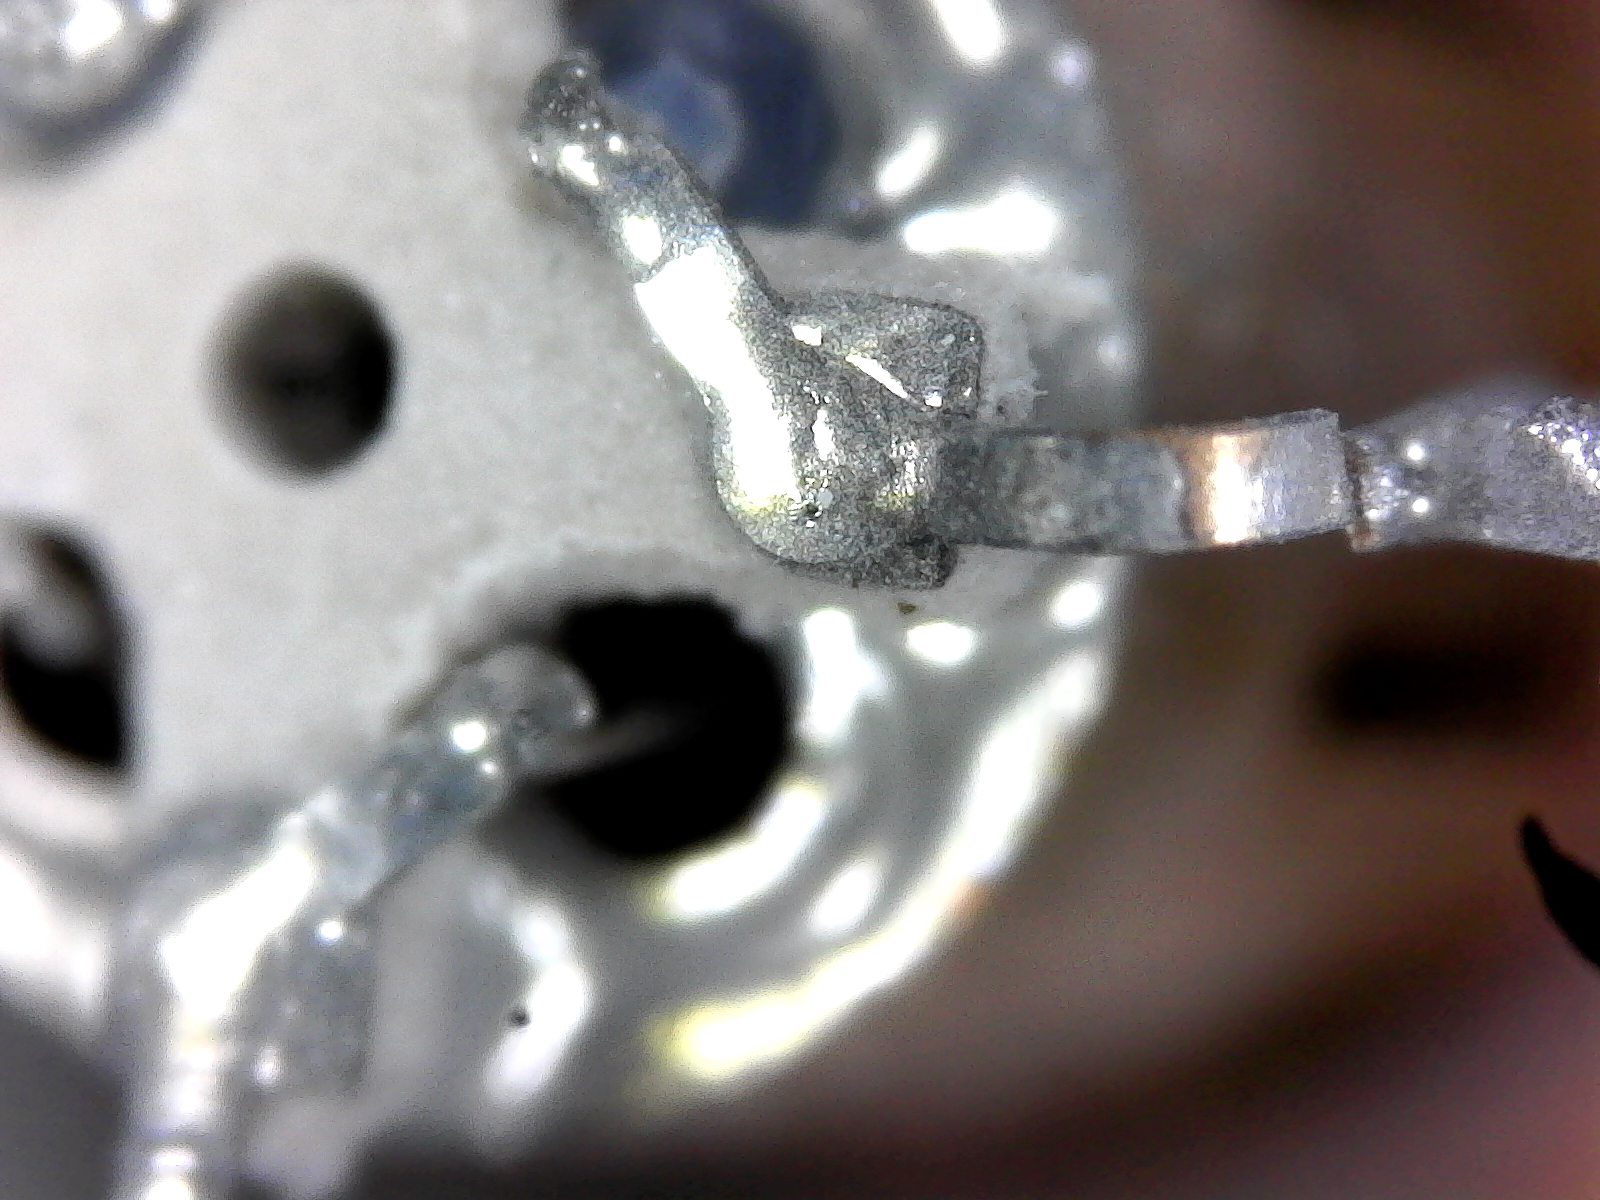
\includegraphics[width=1\linewidth]{../013" "(1H)/1H-3.jpg}
        \caption{}
        \label{fig:}
   	\end{subfigure}
   
 	\vspace{1mm}
   
        \begin{subfigure}[t]{0.475\textwidth}
        \centering
        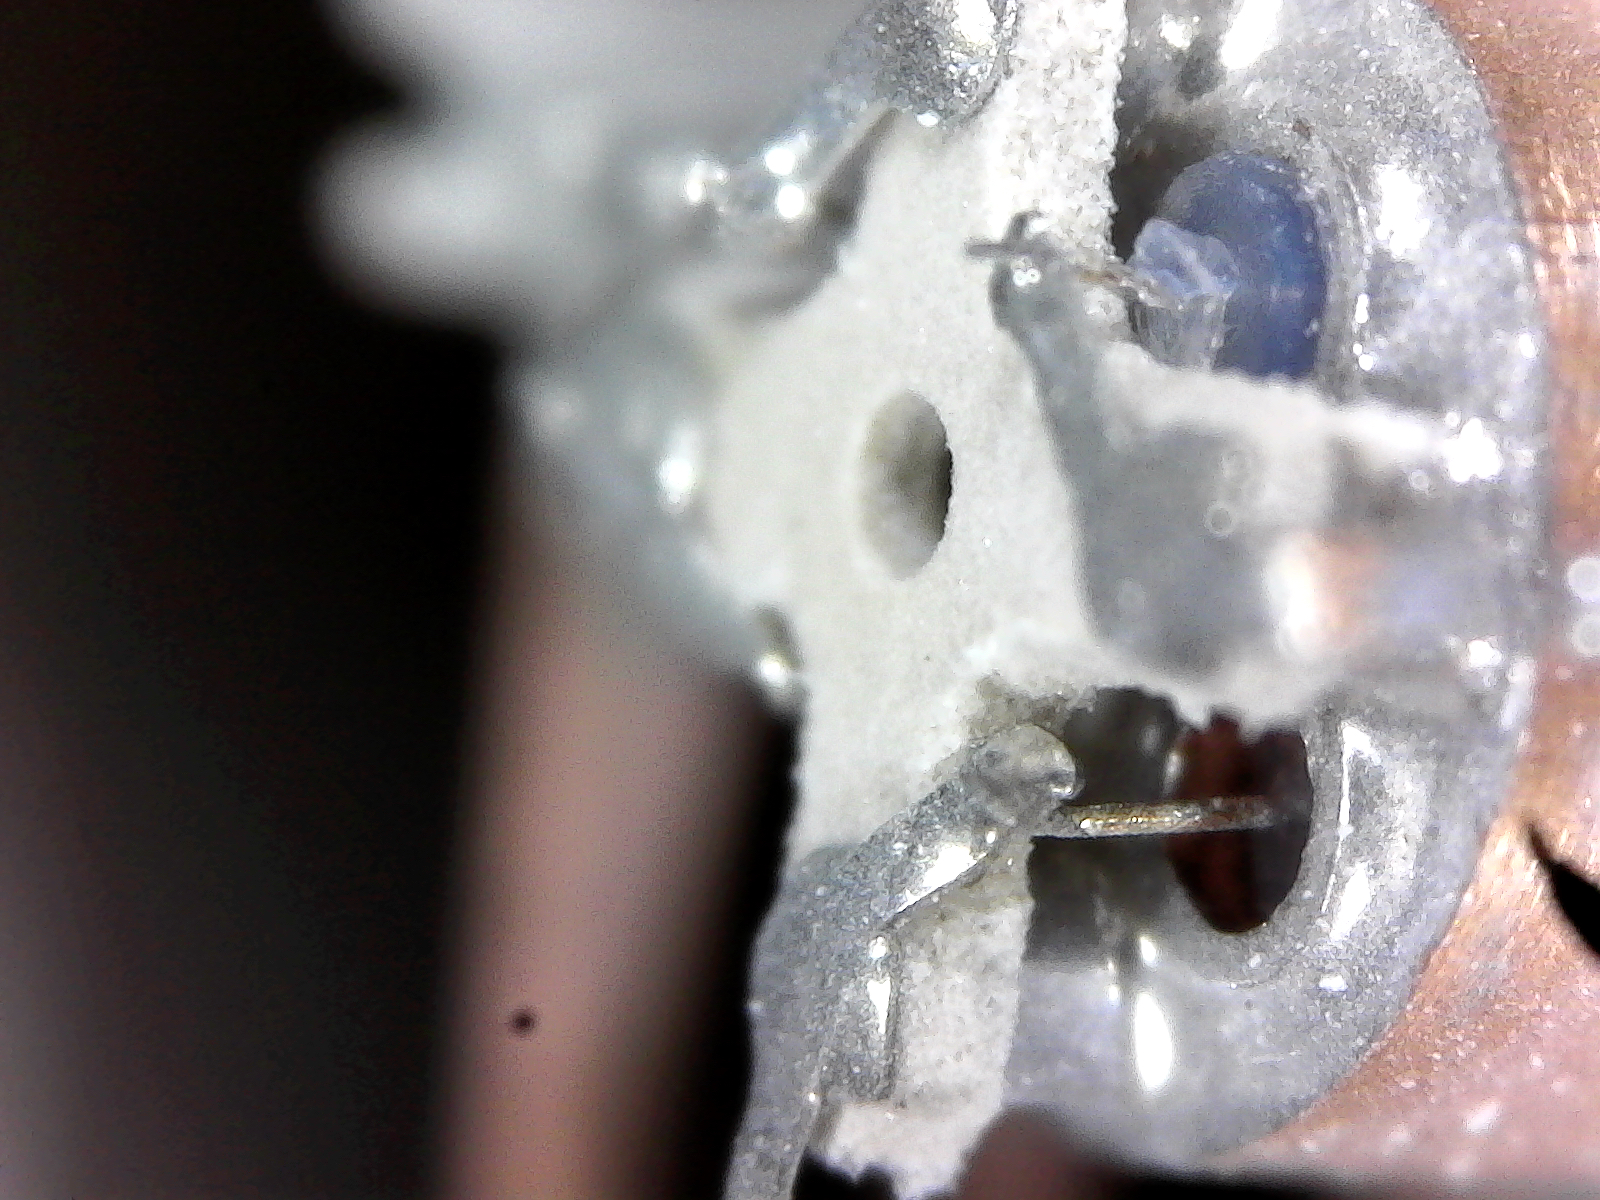
\includegraphics[width=1\linewidth]{../013" "(1H)/1H-5.jpg}
        \caption{}
        \label{fig:}
   	 \end{subfigure}
    %~
        \begin{subfigure}[t]{0.475\textwidth}
        \centering
        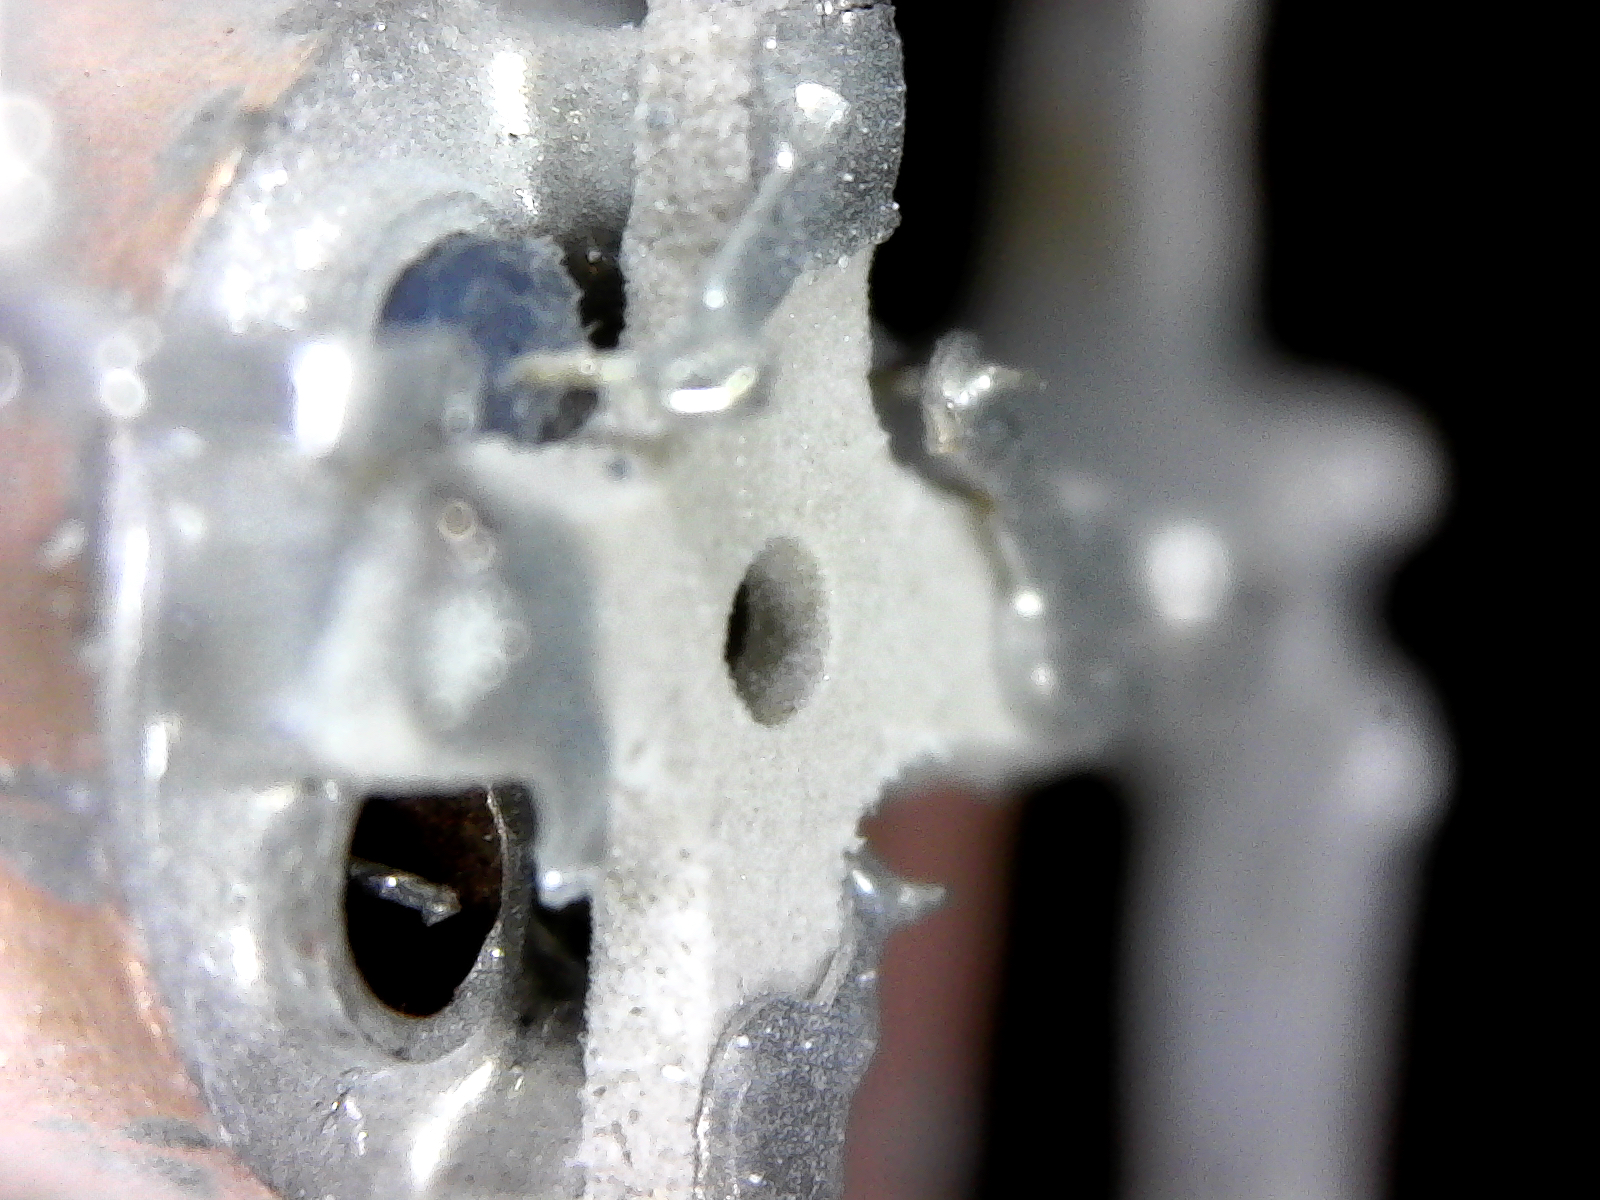
\includegraphics[width=1\linewidth]{../013" "(1H)/1H-6.jpg}
        \caption{}
        \label{fig:}
  	\end{subfigure}  
    %
    \caption{Tip of feed 013 previously installed on 1H. (a) Shows a crack in the tip-link arm next to the capacitor pad. (b) Shows a broken tip-link connection. (c) Shows a retracted coaxial center conductor which is still connected to the tip-link. Although one can see that the tip-link is already bend downwards. (d) Shows the broken connection caused by a retracted coaxial center conductor. }
    \label{fig:inspect-013(1)}
\end{figure}



\newpage
\section{Feed 012 (1K)\\$[$original Antonio Feed$]$}
\label{sec:5}
% ----------------------------------------------------------------

This feed is an original Antonio Feed with no modifications or retrofitted components. The feed has been identified as non operational during the feed system temperature measurements in Oct. 2019 and was switched off afterwards. As part of the tip failure investigation this feed was removed from antenna 1K and inspected. The overall condition of the log-periodic pyramid is shown in Figure \ref{fig:inspect-012(0)}. One can see that there is an extensive amount of dust and particles located at the bottom of the base plate, as well as dust on the log-periodic pyramid itself. The inspection showed that the Rexolite fixture of the feed arms was not sufficient to prevent movement and therefore caused the failure. This also explains the deformation of the feed arms at the tip of the log-periodic pyramid. 

The inspection of the feed tip is shown in Figure \ref{fig:inspect-012(1)} and \ref{fig:inspect-012(2)}. One can see that all coaxial connections are still in place and no sign of coaxial center conductor retraction is visible. However, all four tip-link connections are broken due to the insufficient mechanical support of the Rexolite standoffs. Adding to that, the vibration environment of that feed is unknown, hence it is very likely that the cryocooler is not tuned and therefore the vibrations experienced by the log-periodic feed structure were higher than in the revised feed versions.


\newpage
%
\begin{figure}[H]
   %\thispagestyle{empty}
    \centering
        \begin{subfigure}[t]{0.475\textwidth}
        \centering
        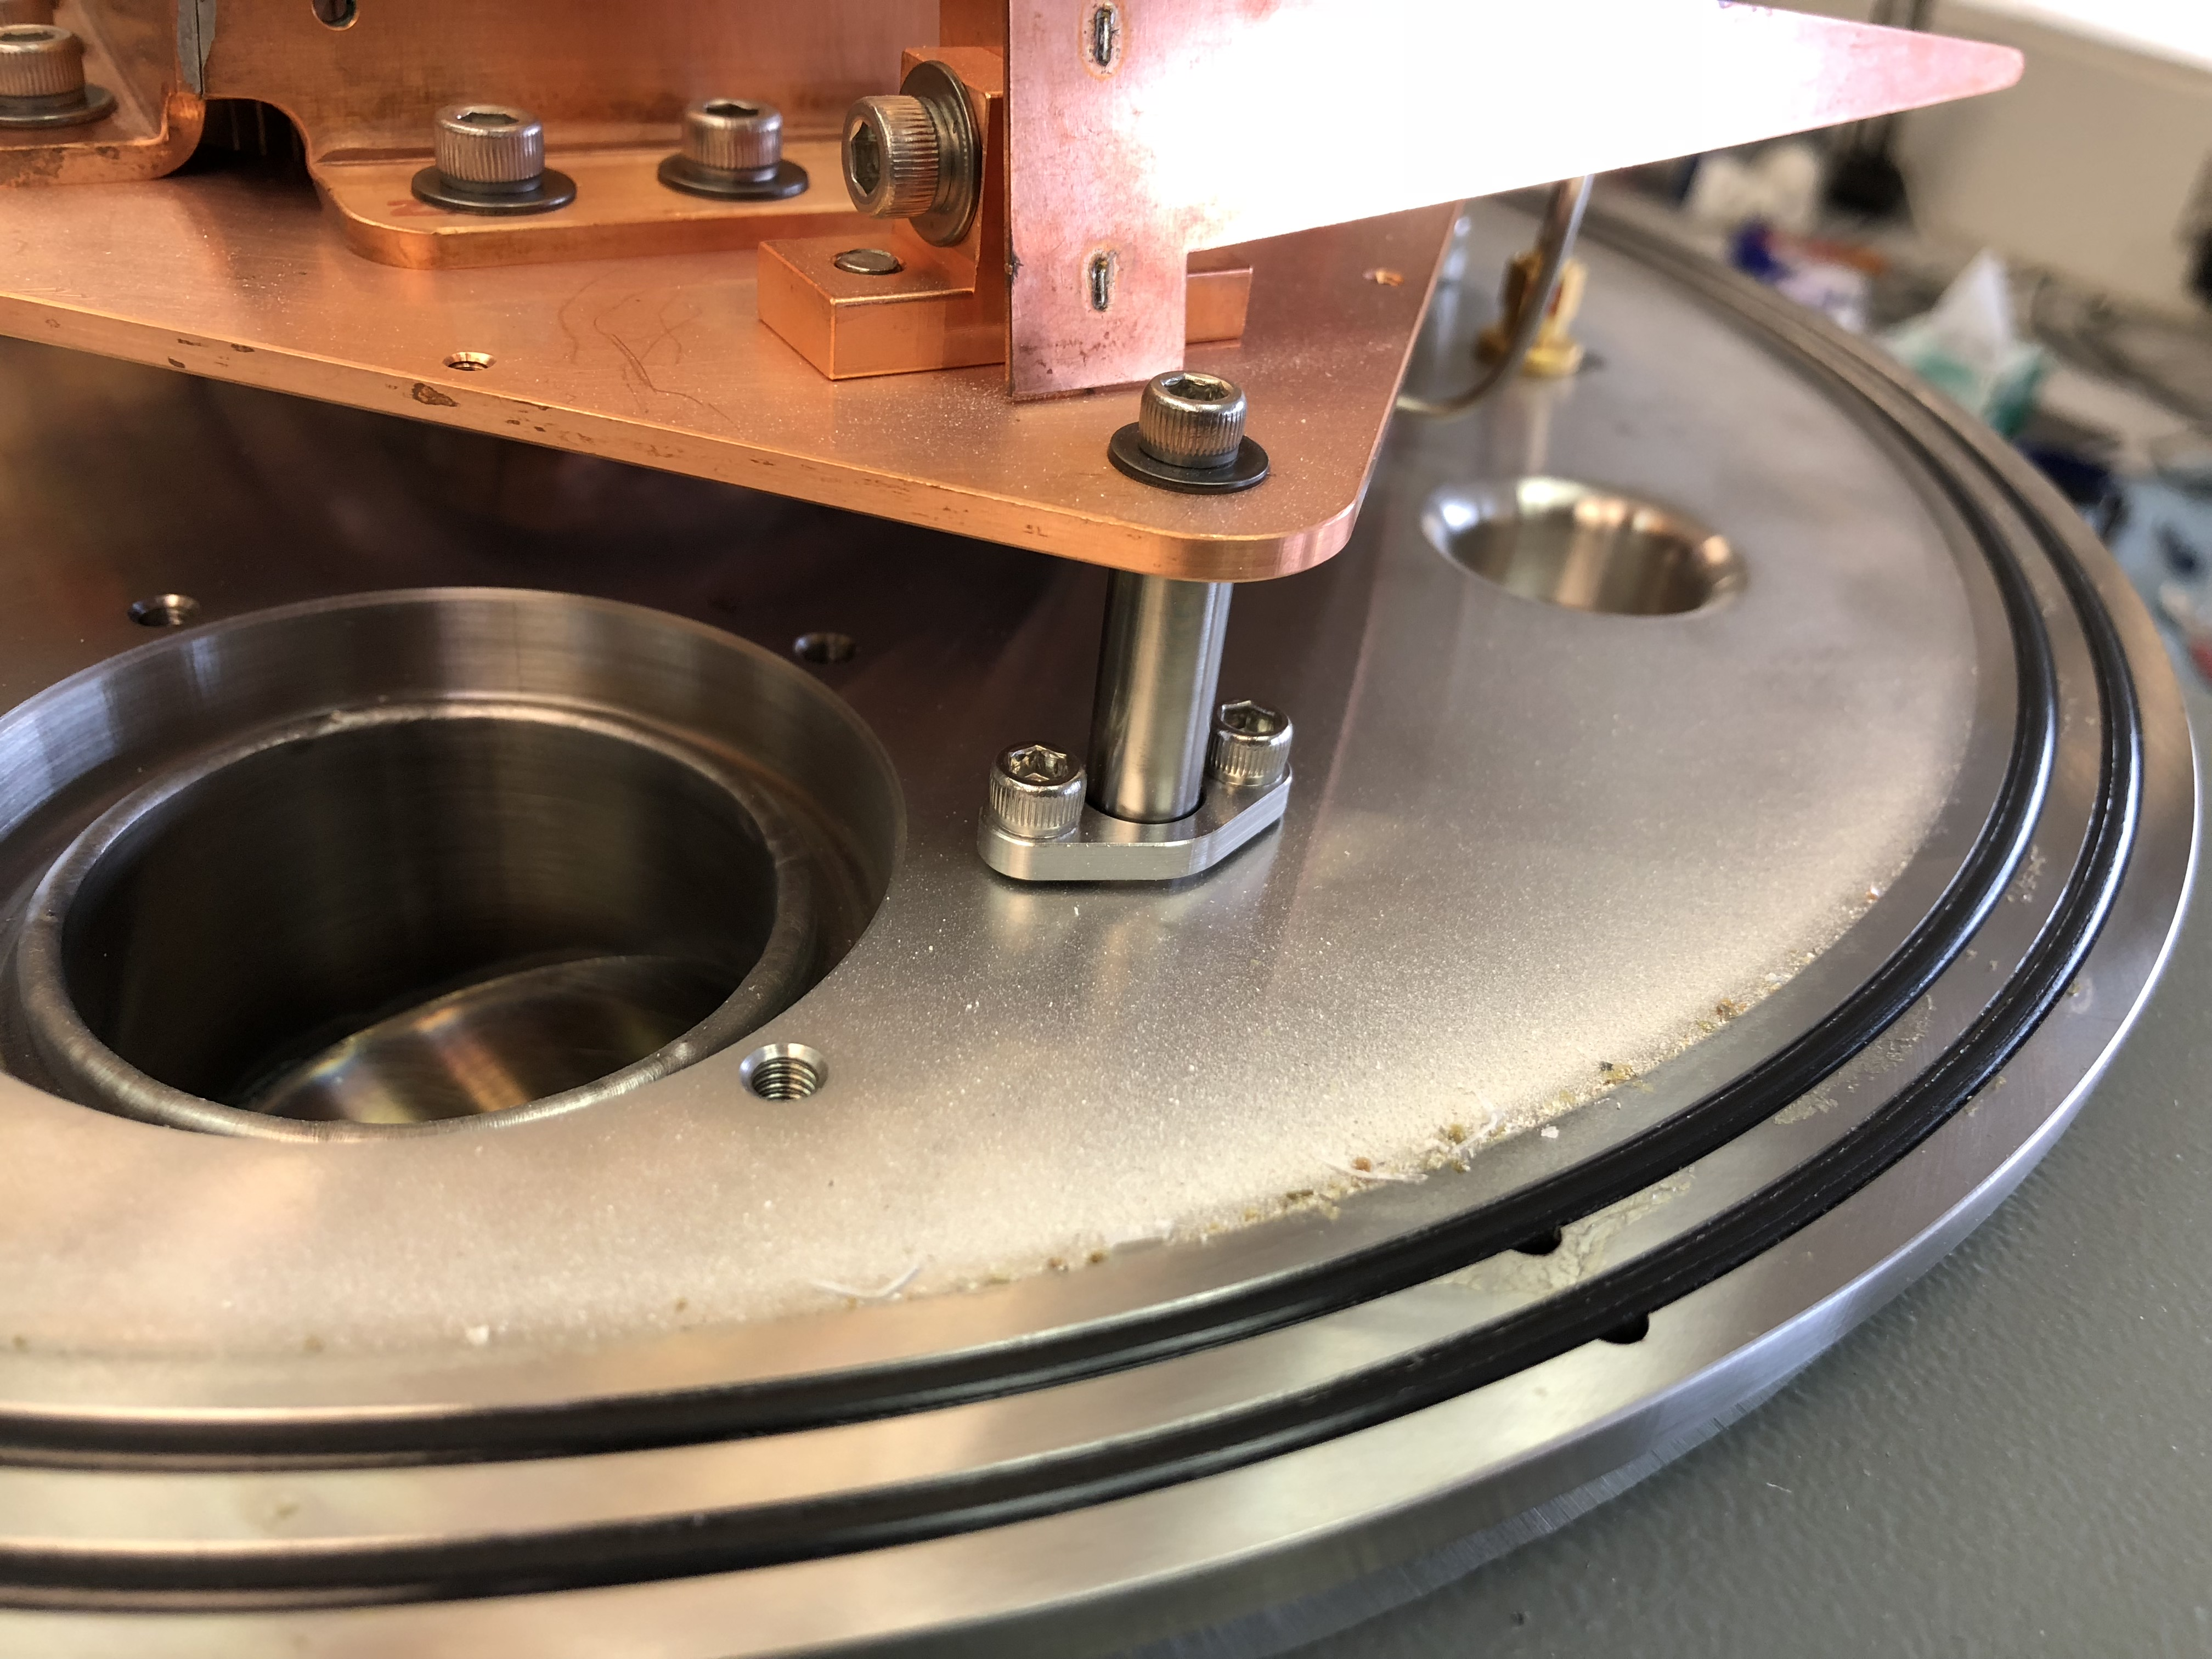
\includegraphics[width=1\linewidth]{../012" "(1K)/IMG_5301.jpg}
        \caption{}
        \label{fig:Tsys-1g}
   	 \end{subfigure}
    %~
        \begin{subfigure}[t]{0.475\textwidth}
        \centering
        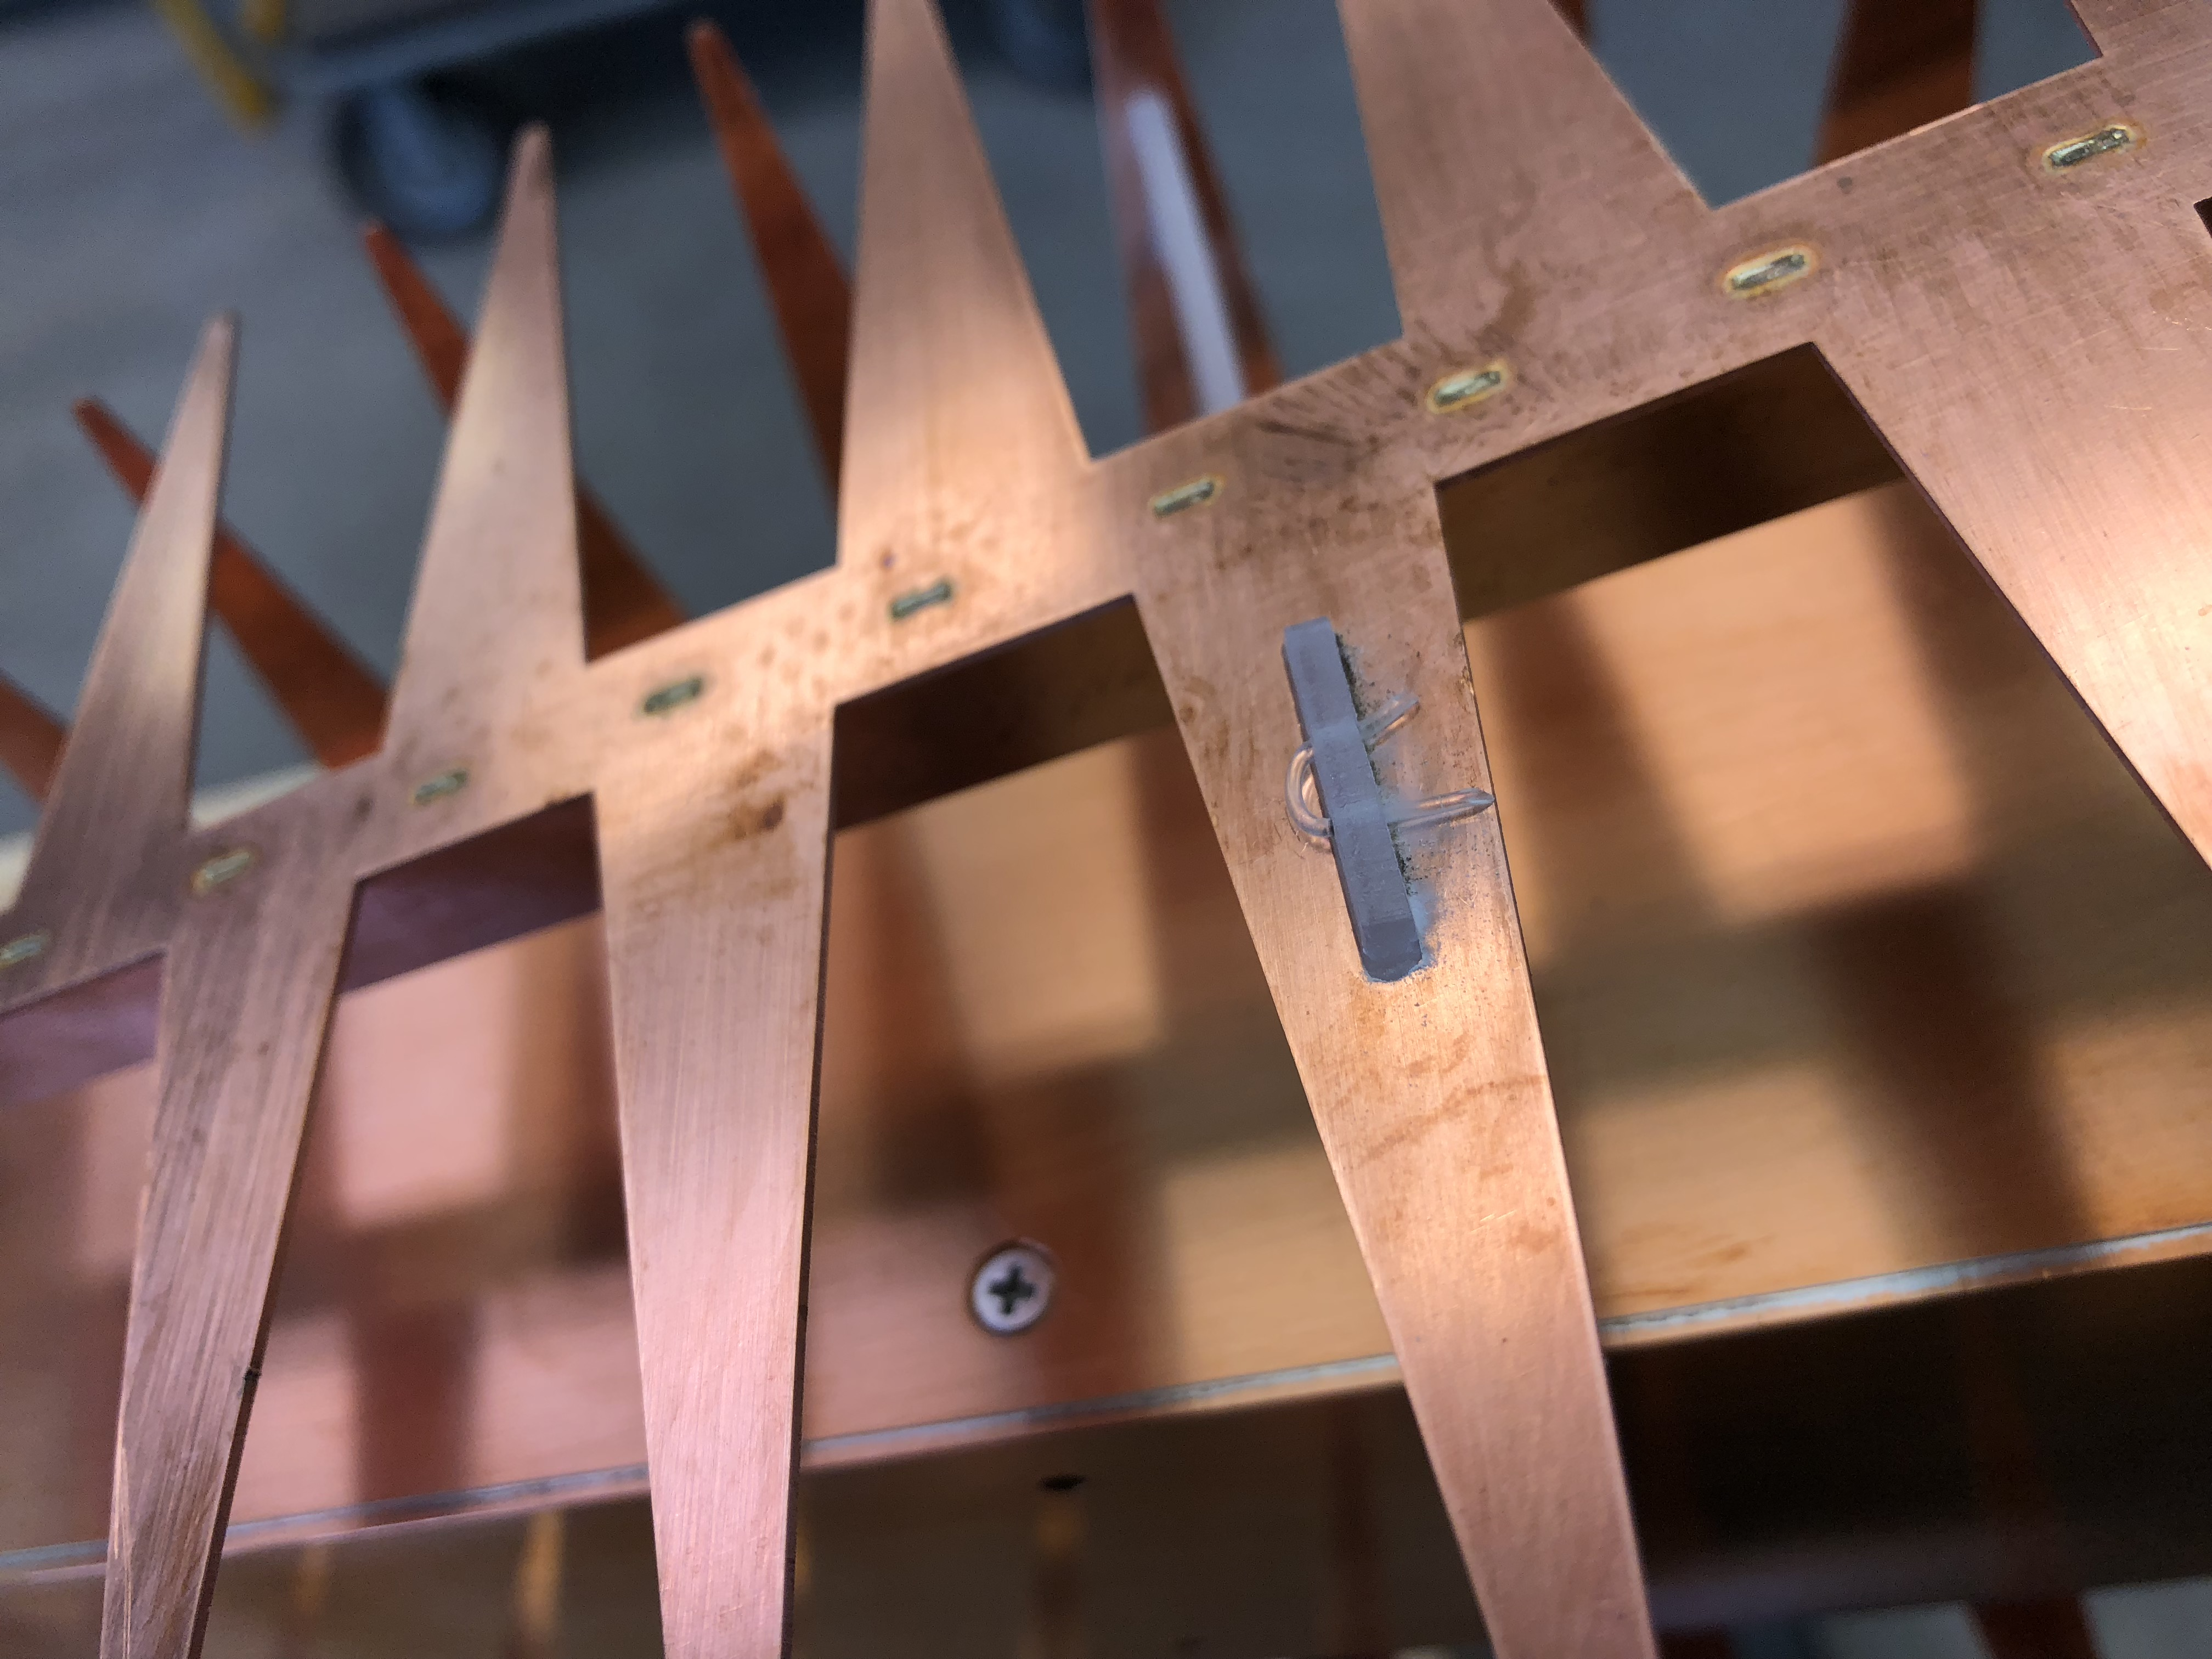
\includegraphics[width=1\linewidth]{../012" "(1K)/IMG_5303.jpg}
        \caption{}
        \label{fig:Y-factor-1g}
   	\end{subfigure}
   
 	%\vspace{1mm}
   
        \begin{subfigure}[t]{0.475\textwidth}
        \centering
        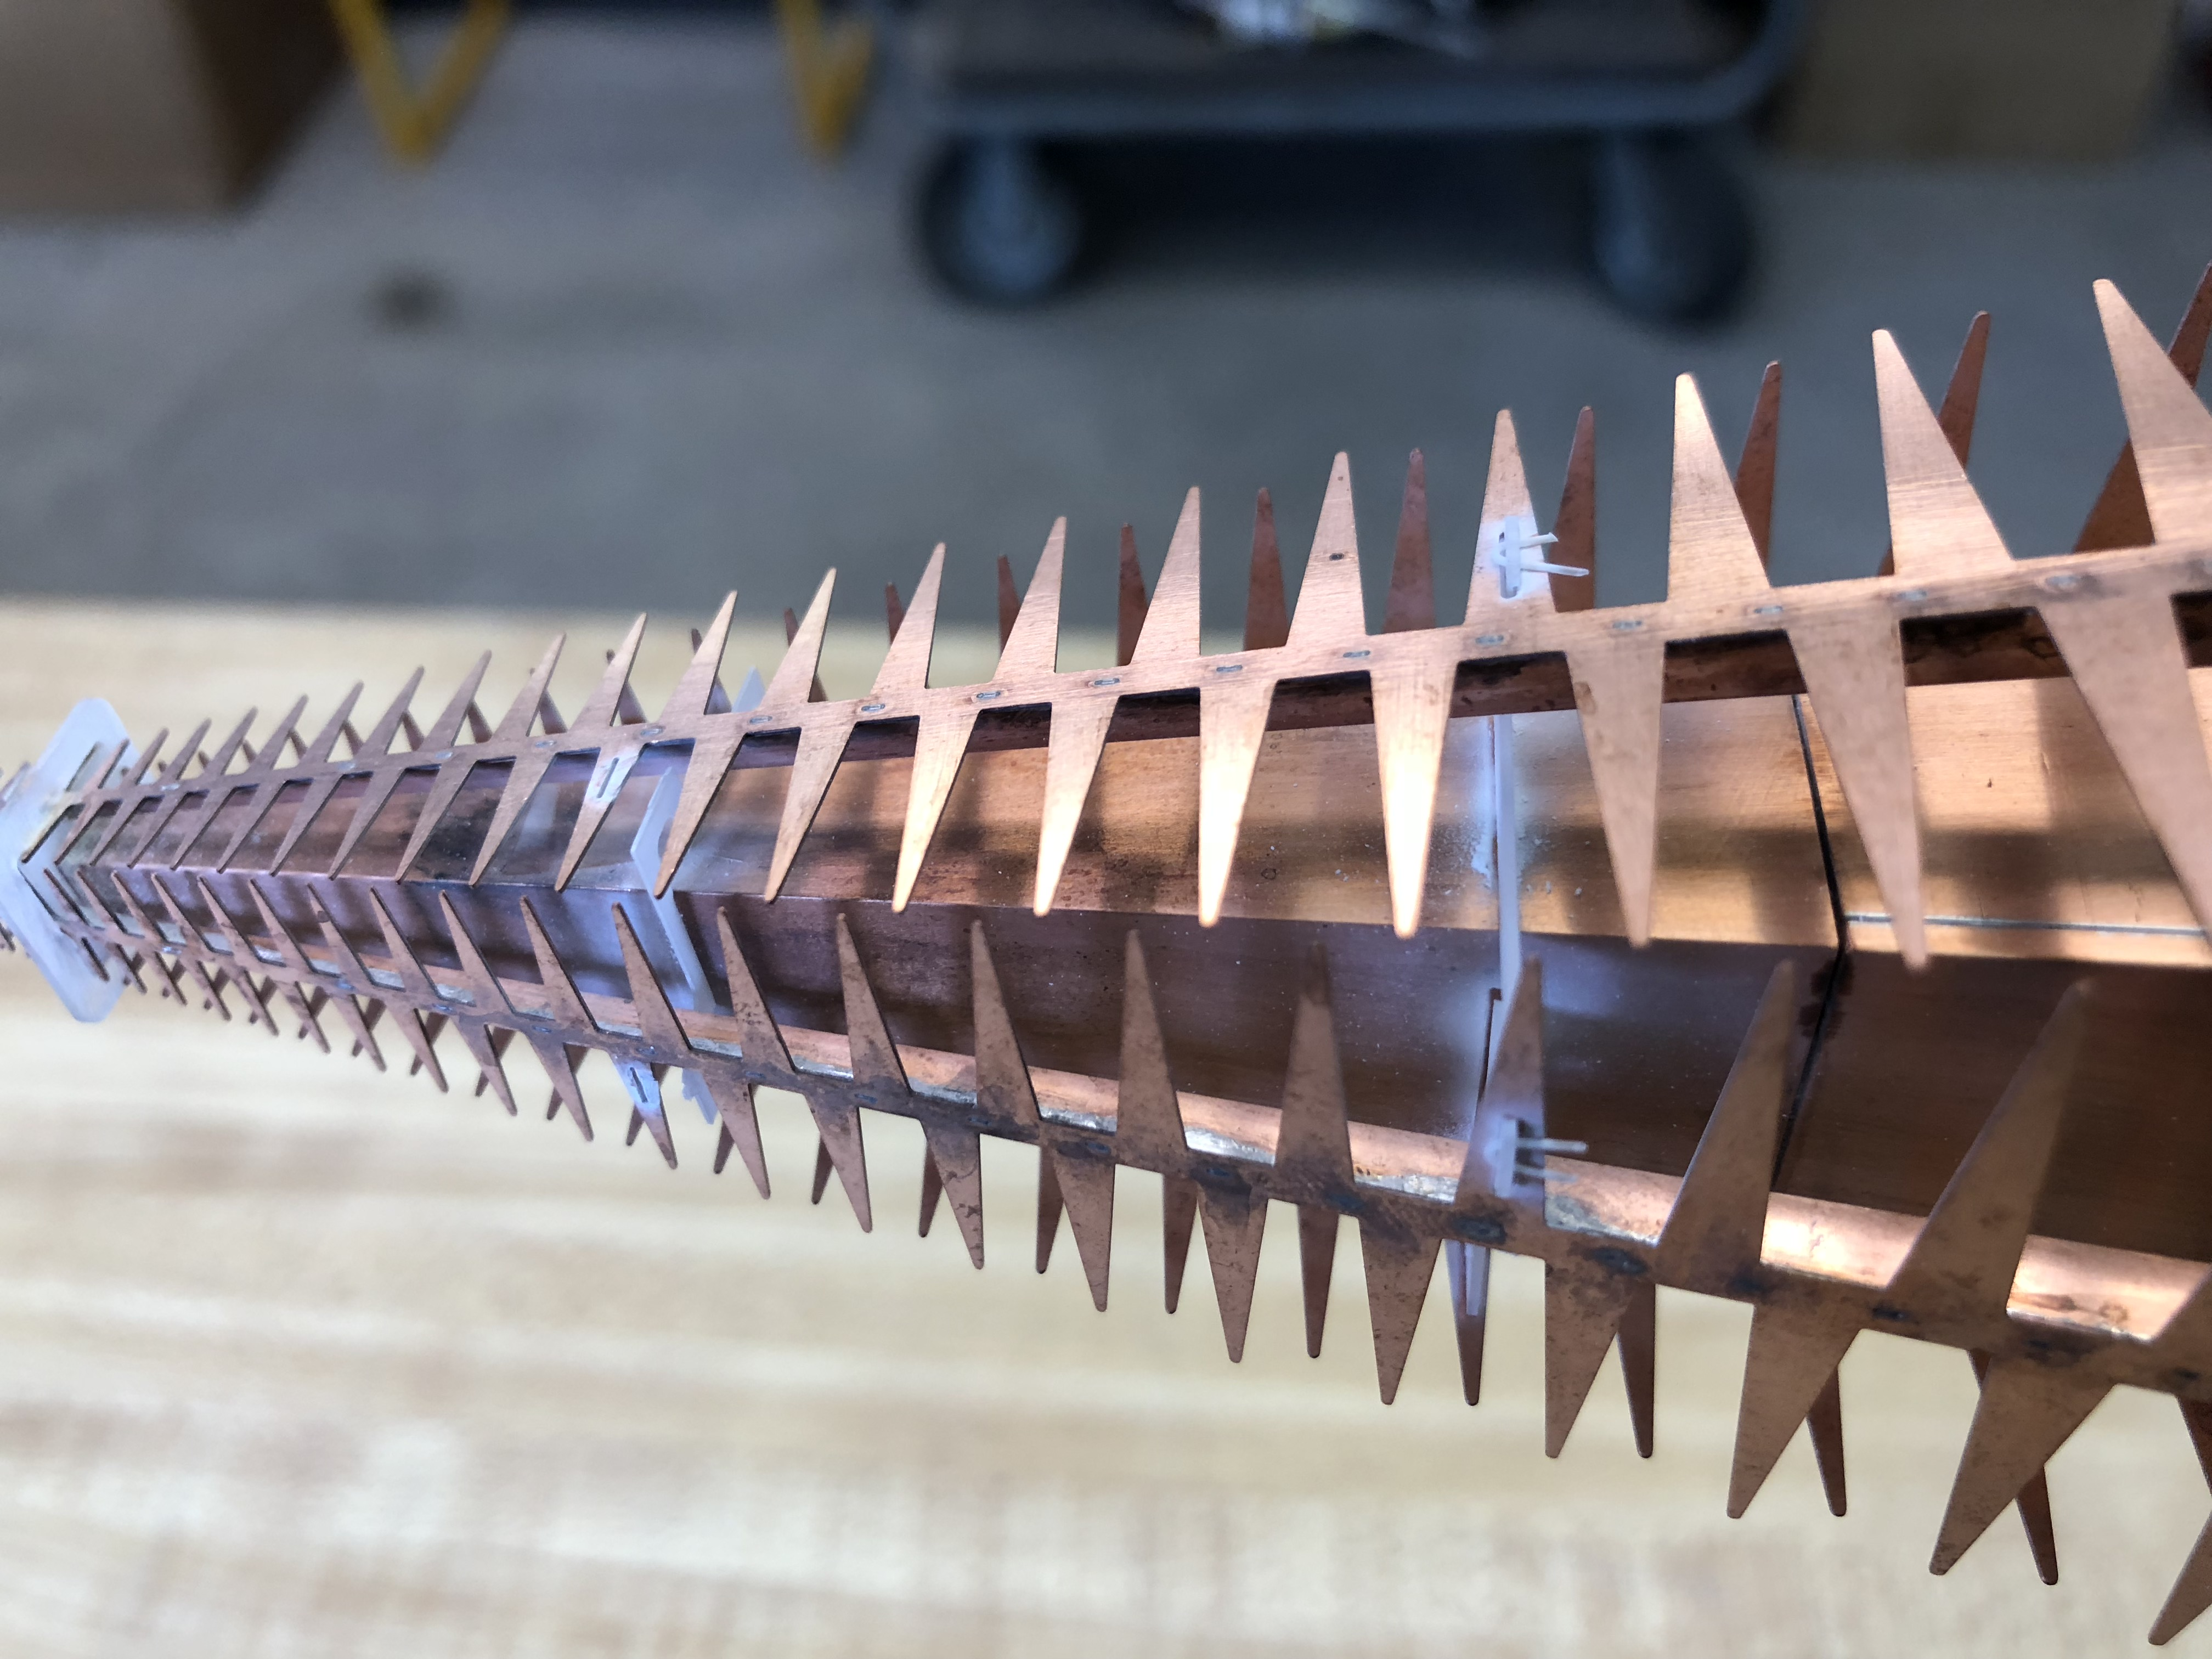
\includegraphics[width=1\linewidth]{../012" "(1K)/IMG_5304.jpg}
        \caption{}
        \label{fig:SpecX-1g}
   	 \end{subfigure}
    %~
        \begin{subfigure}[t]{0.475\textwidth}
        \centering
        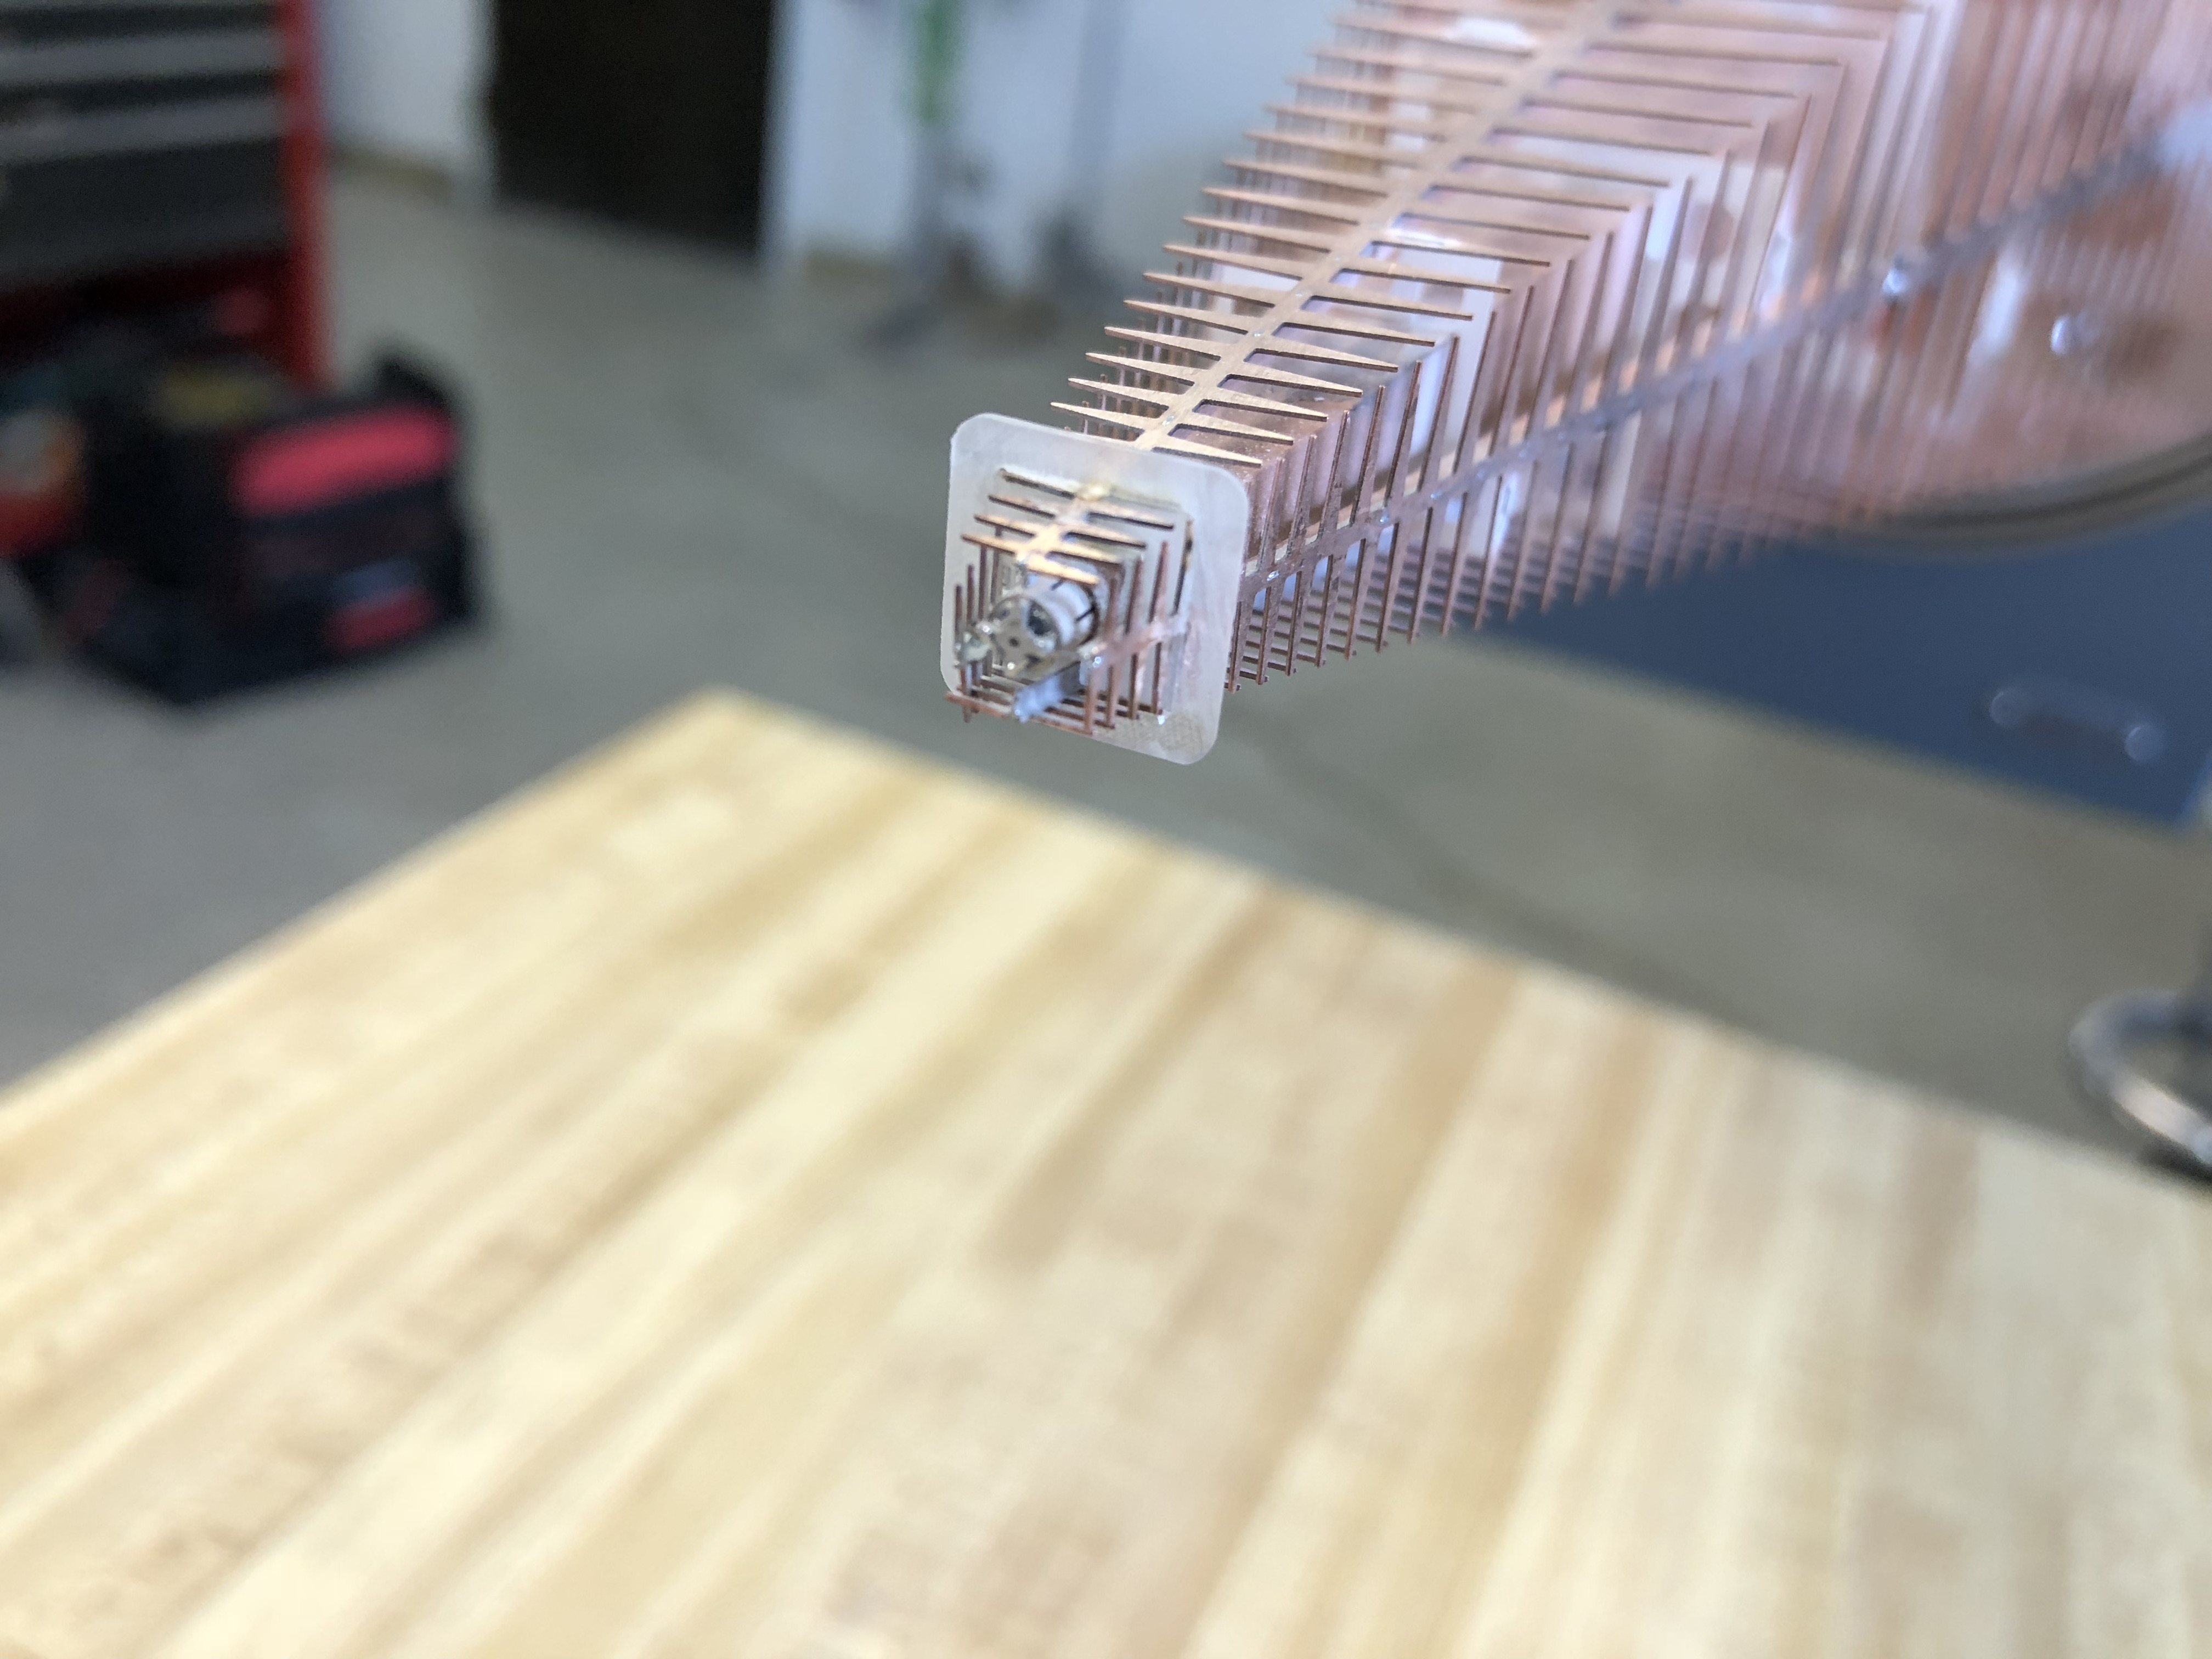
\includegraphics[width=1\linewidth]{../012" "(1K)/IMG_5305.jpg}
        \caption{}
        \label{fig:SpecY-1g}
  	\end{subfigure}  
    %
    \caption{Inspection of the cryostat and log-periodic pyramid of feed 012. }
    \label{fig:inspect-012(0)}
\end{figure}


%
\begin{figure}[H]
\centering{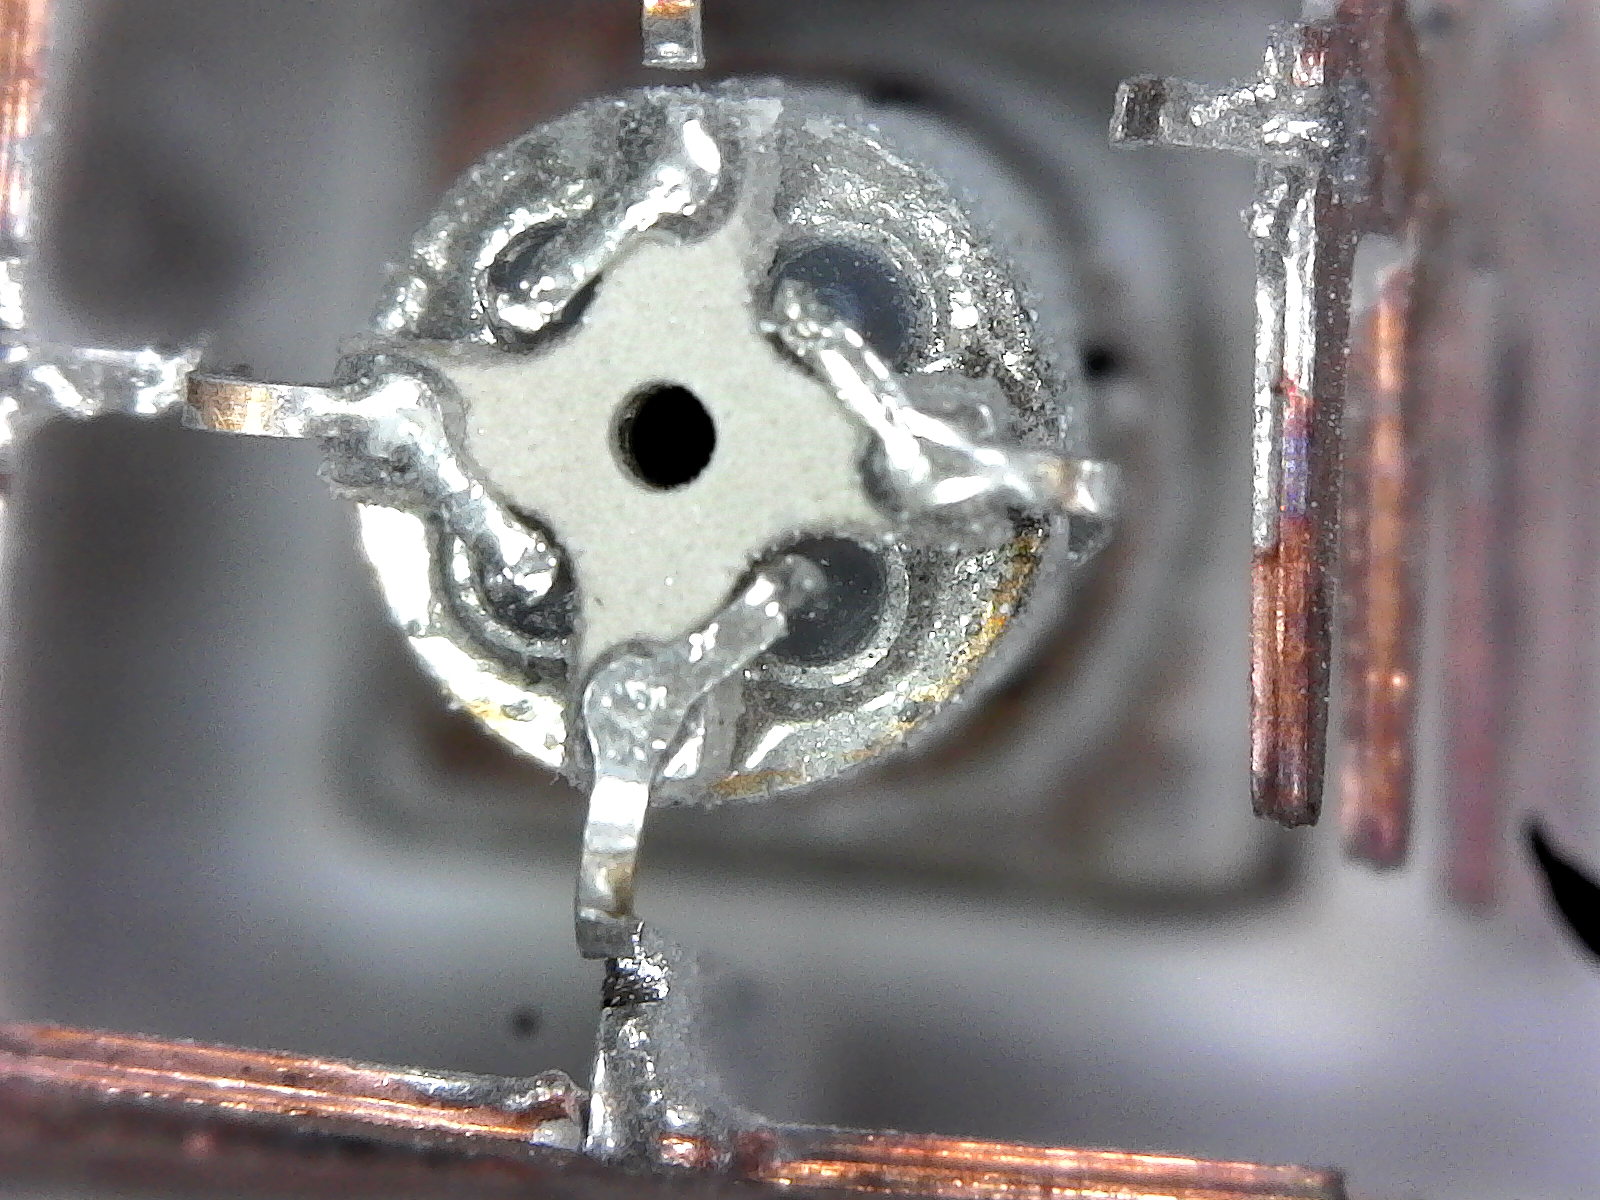
\includegraphics[width=0.69\linewidth]{../012" "(1K)/1K-4.jpg}}
\caption{Top view of the feed 012 tip.}
\label{fig:inspect-012(1)}
\end{figure}
%

\newpage
%
\begin{figure}[H]
   \thispagestyle{empty}
    \centering
        \begin{subfigure}[t]{0.92\textwidth}
        \centering
        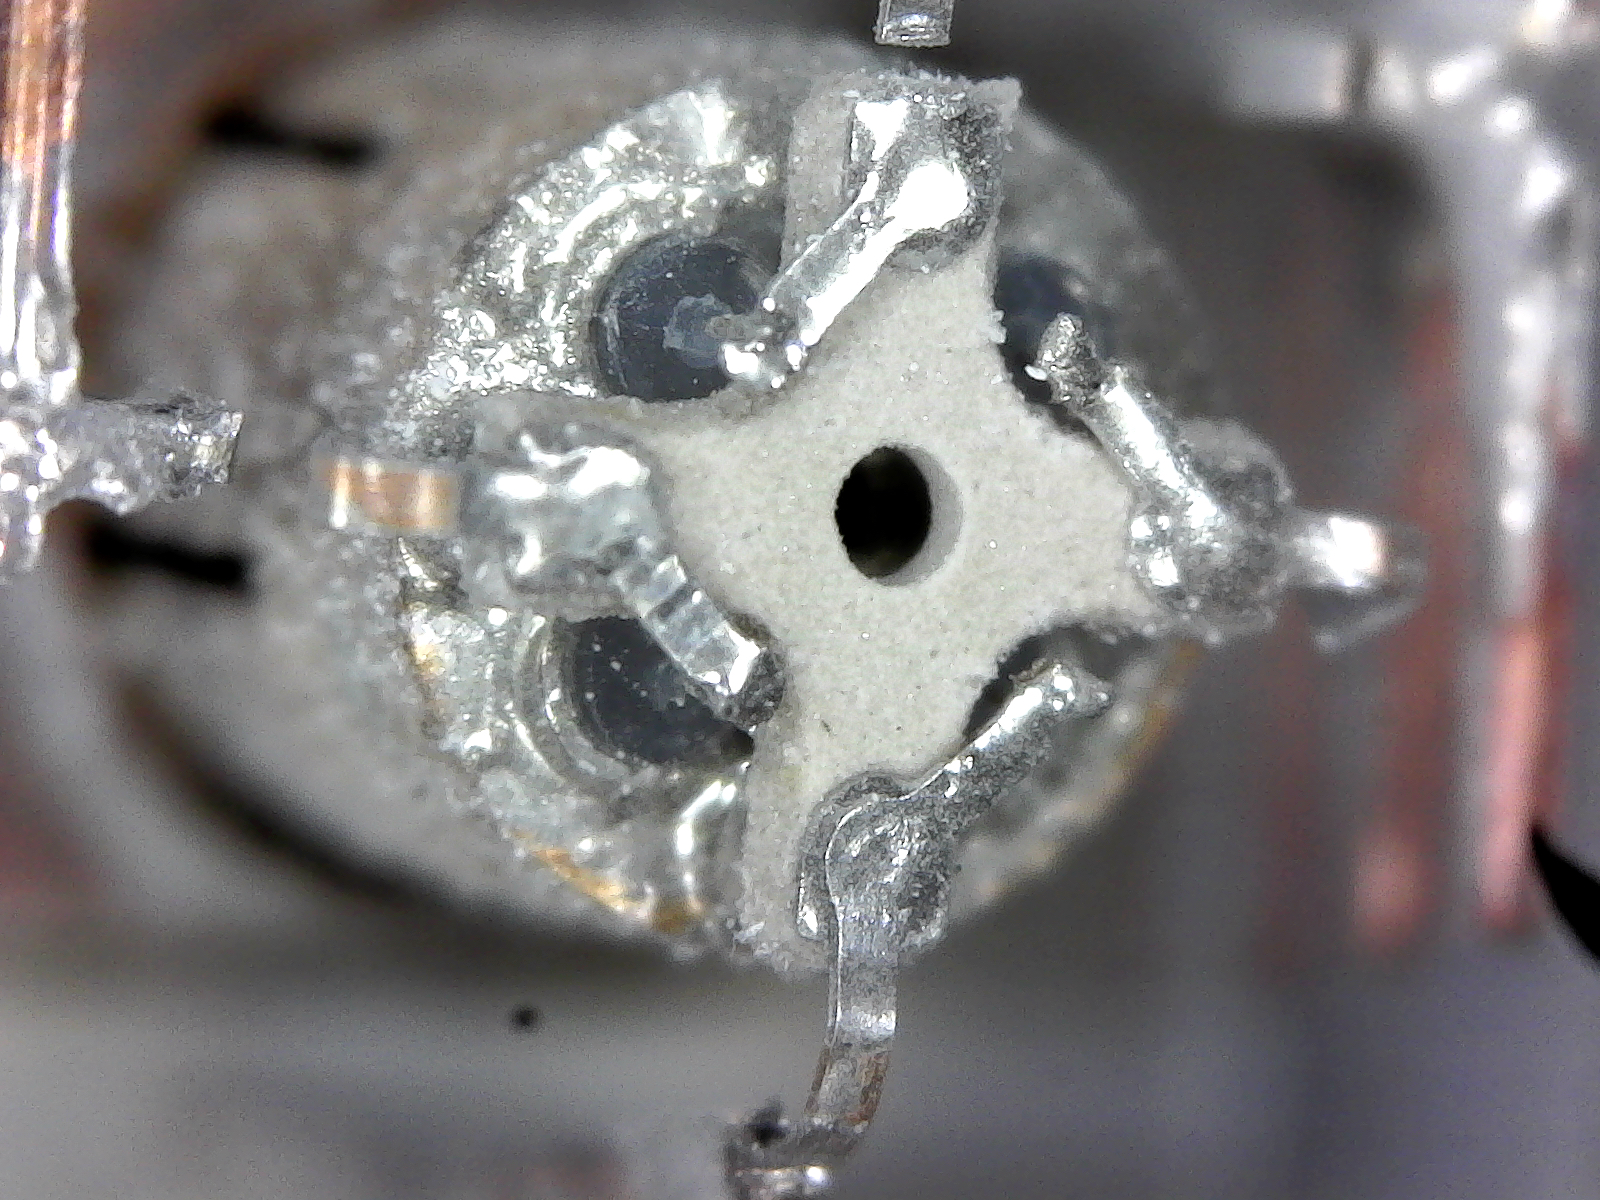
\includegraphics[width=1\linewidth]{../012" "(1K)/1K-1.jpg}
        \caption{}
        \label{fig:Tsys-1g}
   	 \end{subfigure}
	 
        \begin{subfigure}[t]{0.92\textwidth}
        \centering
        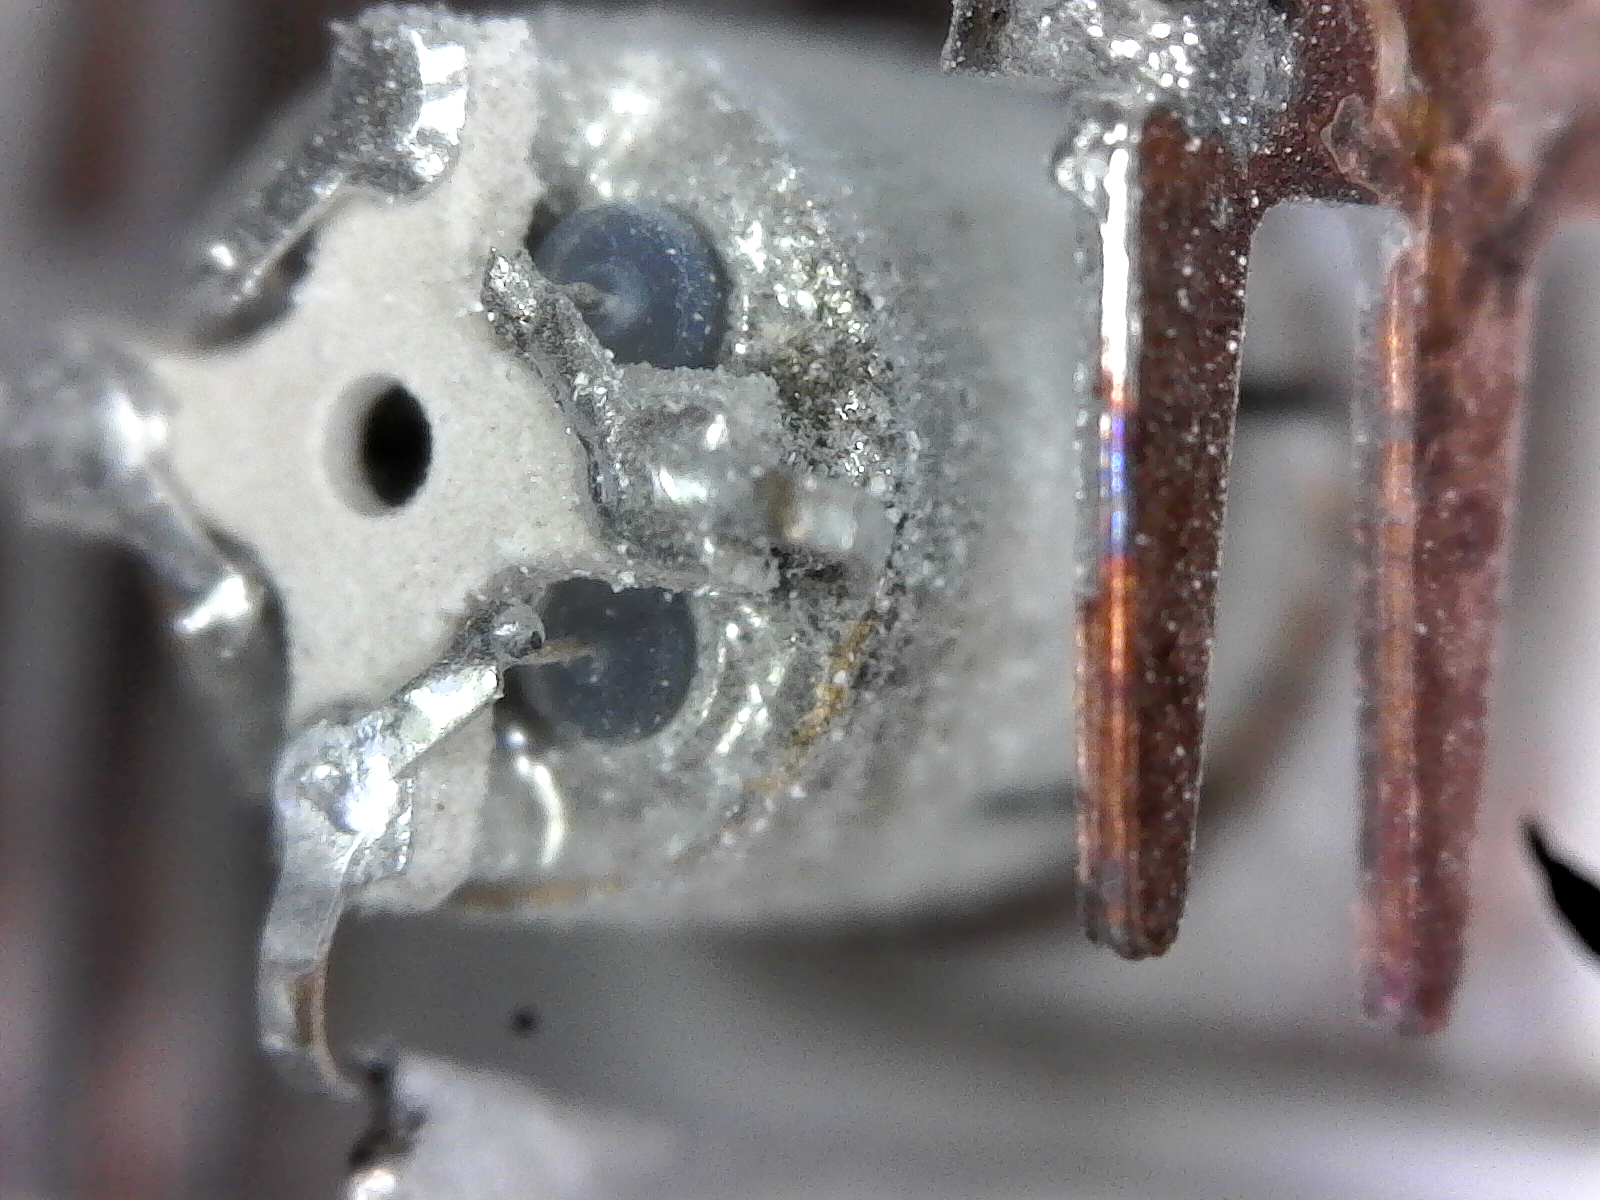
\includegraphics[width=1\linewidth]{../012" "(1K)/1K-3.jpg}
        \caption{}
        \label{fig:SpecX-1g}
   	 \end{subfigure}
    %
    \caption{Tip of feed 012 previously installed on 1K. (a) The left-hand side of the tip, both coaxial connections are still intact, however the tip-link broke off. (b) The right-hand side of the tip shows the same failure mode. }
    \label{fig:inspect-012(2)}
\end{figure}










%----------------------------------------------------------------------------------------
%	BIBLIOGRAPHY
%----------------------------------------------------------------------------------------

%\bibliographystyle{apalike}
%\bibliographystyle{abbrv}

\bibliographystyle{apsrev}
\bibliography{bib_memos}

%----------------------------------------------------------------------------------------



\end{document}
